% !TEX root = ../../book.tex
\chapter{Multivariate Time Series Models\label{ch:ch_mvts}}

The methods developed in this chapter are natural extensions of the methods presented in Chapter~\ref{ch:ch_uvts} in the multivariate setting. But the underlying data is of large dimension and hence they present some unique challenges. These include unwieldy estimation problems as well as making meaningful interpretation of the estimates. But these methods are essential to address portfolio construction and issues related to trading multiple stocks. We want to present some basic tools in multivariate regression and tools for dimension-reduction, which provide a foundation for modeling multiple time series. Although multivariate ARMA models are well-studied in the literature, the focus has been on the multivariate (vector) autoregressive (VAR) models which falls neatly in the framework of multivariate regression with necessary constraints on the regression coefficient matrices that can account for stationarity. Thus a good understanding of multivariate regression will lay a solid foundation for studying VAR models.


In the area of multivariate analysis, there are two broad themes that have emerged over time. One that typically involves exploring the variations in a set of interrelated variables and two, involves investigating the simultaneous relationships between two or more sets of variables. In either case, the themes involve explicit modeling of the relationships or dimension-reduction of the sets of variables. The multivariate regression introduced in Section~\ref{s:s_mr} and its variants are the preferred tools for the parametric modeling and descriptive tools such as principal components or canonical correlations are the tools used for addressing dimension-reduction issues (Section~\ref{sec:s_dr}). Both act as complementary tools and data analyst may want to make use of these tools for a thorough analysis of multivariate data. The methods developed in this chapter will be useful to study cross-sectional momentum, pairs trading, commonality and co-movement, topics that will be followed in subsequent chapters.



% Multivariate Regression
\section{Multivariate Regression \label{s:s_mr}} 

We begin with the general multivariate linear regression model,
	\begin{equation} \label{eqn:5lmyk}
	Y_t = C X_t + \epsilon_t,
	\end{equation}
where $Y_t= (Y_{1t}, \ldots,Y_{mk})'$ is an $m \times 1$ vector of responsive variables and $X_t= (X_{1t}, \ldots, X_{nt})'$ is an $n \times 1$ vector of predictors, $C$ is an $m \times n$ coefficient matrix and $\epsilon_t= (\epsilon_{it}, \ldots, \epsilon_{mt})'$ is the $m \times 1$ vector of random errors. We assume $E(\epsilon_t)= 0$ and $\corr(\epsilon_t)= \Sigma_{\epsilon \epsilon}$ is a $m \times m$ positive definite covariance matrix. The errors are independent over `$t$', the time index. Thus if we arrange the data and error as matrices,
	\begin{equation} \label{eqn:5yyt}
	Y= [Y_1,\ldots,Y_T], \enskip X=[X_1,\ldots,X_T] \text{ and } \epsilon= [\epsilon_1, \ldots,\epsilon_T],
	\end{equation}
and if $e=\text{vec}(\epsilon')$,
	\begin{equation} \label{eqn:5Ee0}
	E(e)=0, \quad \cov(e)= \Sigma_{\epsilon \epsilon} \otimes I_T,
	\end{equation}
where the symbol $\otimes$ signifies the Kronecker's product. 


The unknown parameters in model \eqref{eqn:5lmyk} are the ($mn$) elements of the regression coefficient matrix $C$ and ($m(m+1)/2$) elements of the error covariance matrix $\Sigma_{\epsilon \epsilon}$. These can be estimated by the method of maximum likelihood under the assumption of normality of the $\epsilon_k$ which is equivalent to least squares estimation. Note we can rewrite the model \eqref{eqn:5lmyk} in terms of the data matrices $\mathbf{Y}$ and $\mathbf{X}$ as
	\begin{equation} \label{eqn:rewrite}
	\mathbf{Y} = C \mathbf{X} + \mathbf{\epsilon}.
	\end{equation}
The least squares estimates are obtained by minimizing
	\begin{equation} \label{eqn:minimize}
	e'e= \tr (\epsilon\epsilon')= \tr [(\mathbf{Y} - C\mathbf{X}) (\mathbf{Y} - C \mathbf{X})']= \tr \left[\sum_{t=1}^T \epsilon_t \epsilon_t' \right],
	\end{equation}
where $\tr(A)$ denotes the sum of the diagonal elements of $A$. This yields a unique solution for $C$ as
	\begin{equation} \label{eqn:solution}
	\tilde{C}= \mathbf{Y} \mathbf{X}' (\mathbf{X} \mathbf{X}')^{-1} = \left( \dfrac{1}{T} \mathbf{Y}\mathbf{X}' \right) \left( \dfrac{1}{T} \mathbf{X} \mathbf{X}' \right)^{-1}.
	\end{equation}
Hence, it can be seen from the form of \eqref{eqn:solution} the rows of the matrix $C$ are estimated by the least squares regression of each response variable on the predictor variables as $C'_j= (\mathbf{Y}_j' \mathbf{X})(\mathbf{X}\mathbf{X}')^{-1}$ and therefore the covariances among the response variables do not enter into the estimation. Thus, the multivariate regression is essentially a series of multiple regressions. 


The maximum likelihood estimate of `$C$' under the normality assumption yields the same solution for $C$ as given in \eqref{eqn:solution}. The ML estimator of the error covariance matrix $\Sigma_{\epsilon\epsilon}$ is obtained from the least squares residuals $\hat{\mathbf{\epsilon}}= \mathbf{Y} - \tilde{C} \mathbf{X}$ as $\tilde{\Sigma}_{\epsilon\epsilon}= \frac{1}{T}(\mathbf{Y} - \tilde{C}\mathbf{X})(\mathbf{Y} - \tilde{C} \mathbf{X})' \equiv \frac{1}{T}S$, where $S= \sum_{t=1}^T \hat{\epsilon}_t \hat{\epsilon}_t'$ is the error sum of squares matrix, and $\hat{\epsilon}_t= Y_t - \tilde{C} \mathbf{X}_t$, $t=1,\ldots,T$, are the least squares residual vectors. An unbiased estimator of $\Sigma_{\epsilon\epsilon}$ is obtained as 
	\begin{equation} \label{eqn:5unbiased}
	\overline{\Sigma}_{\epsilon\epsilon} = \dfrac{1}{T-n} \,\hat{\epsilon} \hat{\epsilon}' = \dfrac{1}{T-n} \sum_{t=1}^T \hat{\epsilon}_t \hat{\epsilon}_t'.
	\end{equation}


\noindent\textbf{Inference Properties:} \twomedskip


First, $\tilde{C}$ is an unbiased estimator of $C$, $E(\tilde{C})= C$ and $\cov(\tilde{C}_{(i)}, \tilde{C}_{(j)})= \sigma_{ij} (\mathbf{X}\mathbf{X}')^{-1}$ for $i,j= 1,\ldots, m$, where $\sigma_{ij}$ denotes the $(i,j)$th element of the covariance matrix $\Sigma_{\epsilon\epsilon}$, since $\cov(\mathbf{Y}_{(i)}, \mathbf{Y}_{(j)})= \sigma_{ij} I_T$. The distributional properties of $\tilde{C}$ follow easily from multivariate normality of the error terms $\epsilon_t$. Specifically, we consider the distribution of $\tvec(\tilde{C}')$, where the ``vec'' operation transforms an $m \times n$ matrix into an $mn$-dimensional column vector by stacking the columns of the matrix below each other. 


\setcounter{result}{0}
\begin{result} \label{res:1}
For the model \eqref{eqn:5lmyk} under the normality assumption on the $\epsilon_k$,  the distribution of the least squares estimator $\tilde{C}$ in \eqref{eqn:solution} is that 
	\begin{equation} \label{eqn:distlsq}
	\tvec(\tilde{C}') \sim N(\tvec(C'), \Sigma_{\epsilon\epsilon} \otimes (\mathbf{X} \mathbf{X}')^{-1}).
	\end{equation}
Note, in particular, that this result implies that the $j$th row of $\tilde{C}$, $\tilde{C}_{(j)}'$, which is the vector of least squares estimates of regression coefficients for the $j$th response variable, has the distribution $\tilde{C}_{(j)} \sim N(C_{(j)}, \sigma_{jj}( \mathbf{X} \mathbf{X}')^{-1} )$. The inference on the elements of the matrix $C$ can be made using the result in \eqref{eqn:distlsq}. In practice, because $\Sigma_{\epsilon\epsilon}$ is unknown, a reasonable estimator such as the unbiased estimator in \eqref{eqn:5unbiased} is substituted for the covariance matrix in \eqref{eqn:distlsq}.


We shall indicate the likelihood ratio procedure for testing simple linear hypotheses regarding the regression coefficient matrix. Suppose $\mathbf{X}$ is partitioned as $\mathbf{X}= [\mathbf{X}_1', \mathbf{X}_2']$ and corresponding $C= [C_1, C_2]$, so that the model \eqref{eqn:rewrite} is written as $\mathbf{Y}= C_1 \mathbf{X}_1 + C_2 \mathbf{X}_2 + \mathbf{\epsilon}$, where $C_1$ is $m \times n_1$ and $C_2$ is $m \times n_2$ with $n_1 + n_2= n$. Suppose we want to test the null hypothesis $H_0: C_2= 0$ against the alternative $C_2 \neq 0$. The null hypothesis implies that the predictor variables $\mathbf{X}_2$ do not have any (additional) influence on the response variables $\mathbf{Y}$, given the impact of the variables $\mathbf{X}_1$. Essentially, this involves running two sets of regressions: one with all predictors ($\mathbf{X}$) and the one with the subset of the predictors ($\mathbf{X}_1$). The LR test statistic is $\lambda= U^{T/2}$, where $U= \lvert S\rvert / \lvert S_1 \rvert$, $S= (\mathbf{Y} - \tilde{C} \mathbf{X} )(\mathbf{Y} - \tilde{C} \mathbf{X} )'$ and $S_1= (\mathbf{Y}-\tilde{C}_1 \mathbf{X}_1 )( \mathbf{Y} - \tilde{C}_1 \mathbf{X}_1 )'$. The matrix $S$ is the residual sum of squares matrix from fitting of the full model, while $S_1$ is the residual sum of squares matrix obtained from fitting the reduced model with $C_2=0$ and $\tilde{C}_1= \mathbf{Y} \mathbf{X}_1' (\mathbf{X}_1 \mathbf{X}_1')^{-1}$. It has been shown (see Anderson (1984)~\cite[Chap. 8]{andersontw2}) that for moderate and large sample size $T$, the test statistic 
	\begin{equation} \label{eqn:mathcal}
	\mathcal{M}= -[T - n + (n_2 - m - 1)/2] \log(U)
	\end{equation}
is approximately distributed as Chi-squared with $n_2 m$ degrees of freedom $(\chi_{n_2m}^2)$; the hypothesis is rejected when $\mathcal{M}$ is greater than a constant determined by the $\chi_{n_2m}^2$ distribution. 
\end{result}


Finally, we briefly consider testing the more general null hypotheses of the form $H_0: FC=0$ where $F$ is a known full-rank matrix of dimensions $m_1 \times m$. In the hypothesis $H_0$, the matrix $F$ provides for restrictions in the coefficients of $C$ across the different response variables. Using the LR approach, the likelihood ratio is given by $\lambda= U^{T/2}$ where $U= |S|/|S_1|$ and $S_1= (\mathbf{Y} - \hat{C}\mathbf{X})(\mathbf{Y}  - \hat{C}\mathbf{X})'$ with $\hat{C}$ denoting the ML estimator $C$ obtained subject to the constraint that $f_1C=0$. In fact, it can be shown that the constrained ML estimator under $FC= 0$ can be expressed as
	\begin{equation} \label{eqn:lagconstr}
	\hat{C}= \tilde{C} - SF'(FSF')^{-1} F.
	\end{equation}
From \eqref{eqn:lagconstr}, we therefore have
	\begin{equation} \label{eqn:boldys}
	\mathbf{Y} - \hat{C} \,\mathbf{X}= ( \mathbf{Y} - \tilde{C} \mathbf{X}  ) + SF'(FSF')^{-1} F \tilde{C},
	\end{equation}
where the two terms on the right are orthogonal. We thus readily find that
	\begin{equation} \label{eqn:lastdouble5}
	\begin{split}
	S_1= S + SF'&(FSF')^{-1}( F\tilde{C} (XX') \tilde{C} F' )(FSF')^{-1} FS \equiv S + H,
	\end{split}
	\end{equation}
and $U= 1/\lvert I + S^{-1}H \rvert$ so that the LR test can be based on the eigenvalues of $S^{-1}H$.


The nonzero eigenvalues of the $m \times m$ matrix $S^{-1} H$ are the same as those of the $m_1 \times m_1$ matrix $S_*^{-1} H_*$, where $S_*= FSF'$ and $H_* = FHF' = F \tilde{C} (XX') \tilde{C}' F'$, so that $U^{-1} = \lvert I + S_*^{-1} H_* \rvert= \prod_{i=1}^{m_1} (1 + \hat{\lambda}_i^2 )$, where the $\hat{\lambda}_i^2$ are the eigenvalues of $S_*^{-1} H_*$. Analogous to \eqref{eqn:mathcal}, the test statistic used is $\mathcal{M}= -[T - n + \frac{1}{2}(n - m_1 - 1)]\log(U)$ which has an approximate $\chi_{nm_1}^2$ distribution under $H_0$. Somewhat more accurate approximation of the null distribution of $\log(U)$ is available based on the $F$-distribution, and in some cases (notably $m_1= 1$ or 2) exact $F$-distribution results for $U$ are available (see Anderson (1984)~\cite[Chap. 8]{andersontw2}). However, for most of the applications the large sample $\chi_{nm_1}^2$ approximation for the distribution of the LR statistic $\mathcal{M}$ is normally used. \twomedskip


\noindent \textbf{Prediction:} \twomedskip


Another problem of interest in regard to the multivariate linear regression model \eqref{eqn:5lmyk} is confidence regions for the mean responses corresponding to a fixed value $X_0$ of the predictor variables. The mean vector of responses at $X_0$ is $CX_0$ and its estimate is $\tilde{C}X_0$. Under the assumption of normality of the $\epsilon_k$, it follows that
	\begin{equation} \label{eqn:tcal}
	\mathcal{T}^2= ( \tilde{C }X_0 - CX_0)' \overline{\Sigma}_{\epsilon\epsilon}^{-1} (\tilde{C} X_0 - CX_0) / \{X_0'(\mathbf{X} \mathbf{X}')^{-1}X_0 \}
	\end{equation}
has the Hotelling's $T^2$-distribution with $T - n$ degrees of freedom, Anderson (1984)~\cite[Chap. 5]{andersontw2}. Thus, $\{(T - n - m + 1)/ m(T - n)\} \mathcal{T}^2$ has the $F$-distribution with $m$ and $T - n - m + 1$ degrees of freedom, so that a $100(1 - \alpha)\%$ confidence ellipsoid for the true mean response $CX_0$ at $X_0$ is given by 
	\begin{equation} \label{eqn:52line}
	\begin{split}
	(\tilde{C}X_0 & -CX_0)' \overline{\Sigma}_{\epsilon\epsilon}^{-1} (\tilde{C}X_0 - CX_0) \\
	&\leq \{X_0' (\mathbf{X}\mathbf{X}')^{-1} X_0\} \left[ \dfrac{m(T - n)}{T - n - m + 1} F_{m,T - n - m + 1}(\alpha) \right],
	 \end{split}
	\end{equation}
where $F_{m,T - n - m + 1}(\alpha)$ is the upper 100$\alpha$th percentile of the $F$-distribution with $m$ and $T - n - m + 1$ degrees of freedom. 


A related problem of interest is the prediction of values of a new response vector $Y_0= CX_0 + \epsilon_0$ corresponding to the predictor variables $X_0$, where it is assumed that $Y_0$ is independent of the values $Y_1, \ldots, Y_T$. The predictor of $Y_0$ is given by $\hat{Y}_0= \tilde{C}X_0$, and it follows similarly to the above result \eqref{eqn:tcal} that a $100(1 - \alpha)\%$ prediction ellipsoid for $Y_0$ is
	\begin{equation} \label{eqn:52another2}
	\begin{split}
	(Y_0 & -\tilde{C}X_0)' \overline{\Sigma}_{\epsilon\epsilon}^{-1} (Y_0 - \tilde{C} X_0) \\
	&\leq \{1 + X_0'(\mathbf{X}\mathbf{X}')^{-1} X_0\} \left[ \dfrac{m(T - n)}{T - n - m + 1} F_{m,T - n - m + 1}(\alpha) \right].
	\end{split}
	\end{equation}
The application of Hotelling's $T^2$ in the context of testing related to CAPM model will be discussed later.



% Dimension-Reduction via Reduced-Rank Regression
\section{Dimension-Reduction via Reduced-Rank Regression \label{sec:s_dr}}

In many practical situations, there is a need to reduce the dimensions of the variables and hence for succinct interpretation. A common approach with only one set of variables say, $Y$ or $X$, is to use Principal Components Analysis (PCA), which focuses on finding the linear combination that captures the most variance. Here doing PCA's on $Y$ and on $X$ and then relating them via regression is not optimal. We approach the problem through the assumption of lower rank of the matrix $C$ in model \eqref{eqn:5lmyk}. More formally, in the model $Y_k= CX_k + \epsilon_k$ we assume that with $m < n$,
	\begin{equation} \label{eqn:rankC}
	\text{rank}(C)= r \leq \min(m,n)= m.
	\end{equation}
The rank condition \eqref{eqn:rankC} has two related practical implications. First, with $r < m$ it implies that there are $(m - r)$ linear restrictions on the regression coefficient matrix $C$ of the form
	\begin{equation} \label{eqn:lprimeC}
	l_i' C= 0, \quad i=1,2,\ldots,(m-r)
	\end{equation}
and these restrictions themselves are often not known a priori in the sense that $l_1, \ldots, l_{m-r}$ are unknown, unlike the known constraints $FC=0$ discussed in the last section. Premultiplying \eqref{eqn:5lmyk} by $l_i'$, we have
	\begin{equation} \label{eqn:lprimeY}
	l_i' Y_k= l_i' \epsilon_k.
	\end{equation}
The linear combinations, $l_i'Y_k$, $i=1,2,\ldots,(m-r)$, could be modeled without any reference to the predictor variables $X_k$ and depend only on the distribution of the error term $\epsilon_k$. Otherwise, these linear combinations can be isolated and can be investigated separately. These are called structural relationships in macroeconomics. 


The second implication that is somewhat complementary to \eqref{eqn:lprimeC} is that with assumption \eqref{eqn:rankC}, $C$ can be written as a product of two lower dimensional matrices that are of full rank. Specifically, $C$ can be expressed as
	\begin{equation} \label{eqn:Ceqab}
	C= AB,
	\end{equation}
where $A$ is of dimension $m \times r$ and $B$ is of dimension $r \times n$, but both have rank $r$. Note that the $r$ columns of the left matrix factor $A$ in \eqref{eqn:Ceqab} can be viewed as a basis for the column space of $C$, while the $r$ rows of $B$ form a basis for the row space. The model \eqref{eqn:5lmyk} can then be written as
	\begin{equation} \label{eqn:ykabxk}
	Y_k= A(BX_k) + \epsilon_k, \quad k= 1, 2, \ldots, T,
	\end{equation}
where $BX_k$ is of reduced dimension with only $r$ components. A practical use of \eqref{eqn:ykabxk} is that the $r$ linear combinations of the predictor variables $X_k$ are sufficient to model the variation in the response variables $Y_k$ and there may not be a need for all $n$ linear combinations or otherwise for all $n$ variables, as would be the case when no single predictor variable can be discarded from the full-rank analysis. Hence, there is a gain in simplicity and interpretation through the reduced-rank regression modeling, although from a practitioner point of view one would still need to have measurements on all $n$ predictor variables. But some recent developments on `sparsity' address this issue which will be mentioned briefly later.


For presentation of reduced-rank estimation, we first need an important result known as the Householder-Young or Eckart-Young Theorem (Eckart and Young, 1936~\cite{eckyoung}), which presents the tools for approximating a full-rank matrix by a matrix of lower rank. The solution is related to the singular value decomposition of the full-rank matrix. These results form the basis of most of the well-known dimension-reduction techniques such as principal components. As we shall see, the reduced-rank estimates are obtained as approximation of the full-rank estimate of the regression coefficient matrix. 


\begin{result} \label{res:2}
Let $A$ be a $m \times m$ symmetric matrix with eigenvalues $\lambda_1 \geq \cdots \geq \lambda_m$, and denote the corresponding normalized eigenvectors as $P_1, \ldots, P_m$. The supremum of $\sum_{i=1}^r X_i' A X_i= \tr(X'AX)$, with $X= [X_1, \ldots, X_r]$, over all the sets of $r \leq m$ mutually orthonormal vectors $X_1, \ldots, X_r$ is equal to $\sum_{i=1}^r \lambda_i$ and is attained when the $X_i=P_i$, $i= 1, \ldots, r$. 
\end{result}


The eigenvectors $P_i$ are (essentially) unique, of course, if the eigenvalues $\lambda_i$ are distinct, but the choice of eigenvectors will not be unique if some eigenvalues among the first $r$ are not distinct. An application of the above result in our context follows. 


\begin{result} \label{res:3} 
Let $S$ be a matrix of order $m \times n$ and of rank $m$. The Euclidean norm, $\tr[(S-P)(S-P)']$, is minimum among matrices $P$ of the same order  as $S$ but of rank $r$ ($\leq m$), when $P= MM'S$, where $M$ is $m \times r$ and the columns of $M$ are the first $r$ (normalized) eigenvectors of $SS'$, that is, the normalized eigenvectors corresponding to the $r$ largest eigenvalues of $SS'$. 
\end{result}


\noindent\textbf{Remark (Singular Value Decomposition).} The positive square roots of the eigenvalues of $SS'$ are referred to as the singular values of the matrix $S$. In general, an $m \times n$ matrix $S$, of rank $s$, can be expressed in a \emph{singular value decomposition} as $S= V \Lambda U'$, where $\Lambda= \diag(\lambda_1, \ldots, \lambda_s)$ with $\lambda_1^2 \geq \cdots \geq \lambda_s^2 > 0$ being the nonzero eigenvalues of $SS'$, $V= [V_1, \ldots, V_s]$ is an $m \times s$ matrix such that $V' V= I_s$, and $U= [U_1, \ldots, U_s]$ is $n \times s$ such that $U'U= I_s$. The columns $V_i$ are the normalized eigenvectors of $SS'$ corresponding to the $\lambda_i^2$, and $U_i= \frac{1}{\lambda_i}S'V_i$, $i=1, \ldots, s$. \twomedskip


The ML estimation of model \eqref{eqn:ykabxk}, assuming the $\epsilon_k$ are independent and identically distributed (iid), following a multivariate normal distribution with mean 0 and covariance matrix $\Sigma_{\epsilon\epsilon}$, the solution is given as 
	\begin{equation} \label{eqn:covarmatrixsol}
	\hat{A}^{(r)}= \Gamma^{-1/2} [\hat{V}_1, \ldots, \hat{V}_r], \quad \hat{B}^{(r)}[ \hat{V}_1, \ldots, \hat{V}_r]' \Gamma^{1/2} \hat{\Sigma}_{yx} \hat{\Sigma}_{xx}^{-1},
	\end{equation}
where $\hat{\Sigma}_{yx}= (1/T) \mathbf{Y} \mathbf{X}'$, $\hat{\Sigma}_{xx}= (1/T) \mathbf{X} \mathbf{X}'$, and $\hat{V}_j$ is the eigenvector that corresponds to the $j$th largest eigenvalue $\hat{\lambda}_j^2$ of $\Gamma^{1/2} \hat{\Sigma}_{yx} \hat{\Sigma}_{xx}^{-1} \hat{\Sigma}_{xy}\Gamma^{1/2}$, with the choice $\Gamma= \tilde{\Sigma}_{\epsilon\epsilon}^{-1}$. The solution is based on the singular value decomposition of the standardized regression coefficient matrix $\tilde{\Sigma}_{\epsilon\epsilon}^{-1/2} \tilde{C} \hat{\Sigma}_{xx}^{1/2}$, where $\tilde{C}$ is the least-square estimate of full-rank $C$. The estimates of the constraints, $l_j$'s are obtained from the smallest $(m-r)$ eigenvalues of the same matrix and scaled as, $\hat{l}_j' = \hat{V}_j' \, \Gamma^{1/2}$. 


It should be mentioned, perhaps, that estimation results are sensitive to the choice of scaling of the response variables $Y_k$, and in applications it is often suggested that the component variables $y_{ik}$ be standardized to have unit variances before applying the LS procedure. \twomedskip


\noindent \textbf{Relation to Other Dimension-Reduction Methods} \twomedskip


\noindent\textbf{Principal Component Analysis (PCA)} \twomedskip


\noindent Principal component analysis, originally developed by Hotelling (1933)~\cite{hotelling33}, is concerned with explaining the covariance structure of a large number of variables through a small number of linear combinations of the original variables. Although the two objectives of the PCA data reduction and interpretation which coincide with the objectives of the reduced-rank regression, a major difference is that the principal components are descriptive tools that do not usually rest on any modeling or distributional assumptions. 


Let the $m \times 1$ random vector $Y$ have the covariance matrix $\Sigma_{yy}$ with eigenvlaues $\lambda_1^2 \geq \lambda_2^2 \geq \cdots \geq \lambda_m^2 \geq 0$. Consider the linear combinations $y_1^*= l_1' Y, \ldots, Y_m^* = l_m' Y$, normalized so that $l_i' l_i=1$, $i=1, \ldots, m$. These linear combinations have $\var(y_i^*)= l_i' \Sigma_{yy} l_i$, $i= 1, 2, \ldots, m$, and $\cov(y_i^*,y_j^*)= l_i' \Sigma_{yy} l_j$, $i,j= 1, 2, \ldots, m$. In a principal component analysis, the linear combinations $y_i^*$ are chosen so that they are not correlated but their variances are as large as possible. That is, $y_1^*= l_1' Y$ is chosen to have the largest variance among linear combinations $l_1' l_1= 1$, $y_2^*= l_2' Y$ is chosen to have the largest variance subject to $l_2 l_2=1$ and the condition that $\cov(y_2^*,y_1^*)= l_2' \Sigma_{yy}l_1=0$, and so on. It can be easily shown from Result 1 that the $l_i$'s are chosen to be the (normalized) eigenvectors that correspond to the eigenvalues $\lambda_i^2$ of the matrix $\Sigma_{yy}$, so that the normalized eigenvectors satisfy $l_i' \Sigma_{yy}l_i= \lambda_i^2 \equiv \var(y_i^*)$. Often, the first $r$ ($r<m$) components $y_i^*$, corresponding to the $r$ largest eigenvalues, will contain nearly most of the variation that arises from all $m$ variables. For such cases, in studying variations of $Y$, attention can be directed on these $r$ linear combinations resulting in a reduction in dimension of the variables involved. 


The principal component problem can be represented as a reduced-rank problem, in the sense that a reduced-rank model can be written for this situation as
	\begin{equation} \label{eqn:ykabyk}
	Y_k= ABY_k + \epsilon_k,
	\end{equation}
with $X_k \equiv Y_k$. From the solutions of Result~\ref{res:2}, by setting $\Gamma= I_m$, we have $A^{(r)}= [V_1, \ldots, V_r]$ and $B^{(r)}= V'$ because $\Sigma_{yx}= \Sigma_{yy}$. The $V_j$'s refer to the eigenvectors of $\Sigma_{yy}$. Thus, a correspondence is easily established. The $l_i$ in PCA are the same as the $V_i$ that result from the solution for the matrices $A$ and $B$ in \eqref{eqn:ykabyk}. If both approaches provide the same solutions, one might ask, then, what is the advantage of formulating the principal component analysis in terms of reduced-rank regression model. The inclusion of the error term $\epsilon_k$ appear to be superfluous but the model \eqref{eqn:ykabyk} provides a useful framework to perform the residual analysis to detect outliers, influential observations, and so on, for the principal components method. \twomedskip


\noindent \textbf{Canonical Correlation Analysis:} \twomedskip


\noindent Canonical correlation analysis was introduced by Hotelling~(1935, 1936)~\cite{hotelling35,hotelling36} as a method of summarizing relationships between two sets of variables. The objective is to find that linear combination of one set of variables which is most highly correlated with any linear combination of a second set of variables. The technique has received attention from theoretical statisticians but because of difficulty in interpretation of the canonical variates, its use is not widespread in applications. By exploring the connection between the reduced-rank regression and canonical correlations, we provide an additional method of interpreting the canonical variates. Because the role of any descriptive tool such as canonical correlations is in better model building, the connection we display below provides an avenue for interpreting and further using the canonical correlations for better model building.


More formally, in canonical correlation analysis, for random vectors $X$ and $Y$ of dimensions $n$ and $m$, respectively, the purpose is to obtain an $r \times n$ matrix $G$ and an $r \times m$ matrix $H$, so that the $r$-vector variates $\xi= GX$ and $\omega= HY$ will capture as much of the covariances between $X$ and $Y$ as possible. The following result summarizes how this is done.


\begin{result} \label{res:4} 
We assume $\Sigma_{yy}$ is nonsingular. Then the $r \times n$ matrix $G$ and the $r \times m$ matrix $H$, with $H \Sigma_{yy}H'= I_r$, that minimize simultaneously all the eigenvalues of $E[(HY-GX)(HY-GX)']$ are given by,
	\begin{equation}
	G= V_*'  \Sigma_{yy}^{-1/2} \Sigma_{yx} \Sigma_{xx}^{-1}, \qquad H= V_*'  \Sigma_{yy}^{-1/2},
	\end{equation}
where $V_*= [V_1^*, \ldots, V_r^*]$ and $V_j^*$ is the (normalized) eigenvector corresponding to the $j$th largest eigenvalue $\rho_j^2$ of the matrix
	\begin{equation} \label{eqn:eigenlargestmatrix}
	R_*= \Sigma_{yy}^{-1/2} \Sigma_{yx} \Sigma_{xx}^{-1} \Sigma_{xy} \Sigma_{yy}^{-1/2}.
	\end{equation}
\end{result}


Denoting by $g_j'$ and $h_j'$ the $j$th rows of the matrices $G$ and $H$, respectively, the $j$th pair of canonical variates are defined to be $\xi_j= g_j' X$ and $\omega_j= h_j' Y$, $j= 1, 2, \ldots, m$ ($m \leq n$). The correlation between $\xi_j$ and $\omega_j$ is the $j$th canonical correlation coefficient and hence, since $\cov(\xi_j, \omega_j)= {V_j^*}' R_* V_j^*= \rho_j^2$, $\var(\xi_j)= {V_j^*}' R_* V_j^*= \rho_j^2$, and $\var(\omega_j) ={V_j^*}' V_j^*= 1$, we have $\corr(\xi_j, \omega_j)= \rho_j$ and the $\rho_j$'s are the canonical correlations between $X$ and $Y$. The canonical variates possess the property that $\xi_1$ and $\omega_1$ have the largest correlation among all possible linear combinations of $X$ and $Y$, $\xi_2$ and $\omega_2$ have the largest possible correlation among all linear combinations of $X$ and $Y$ that are uncorrelated with $\xi_1$ and $\omega_1$ and so on. We shall compare the Result~\ref{res:3} with the resulting estimate of reduced-rank models. Because $\Sigma_{\epsilon\epsilon}= \Sigma_{yy} - \Sigma_{yx} \Sigma_{xx}^{-1} \Sigma_{xy}$, the correspondence with results for the choice $\Gamma= \Sigma_{yy}^{-1}$ is fairly simple. It can be shown that,
	\begin{equation} \label{eqn:rhojsqlambj}
	\rho_j^2= \lambda_j^2 / (1+\lambda_j^2)
	\end{equation}
and $G$ and $H$ matrices can be obtained from the rescaled versions of $\hat{V}$, used in Result~\ref{res:3}.



% Multiple Time Series Modeling
\section{Multiple Time Series Modeling}


Multiple time series analysis is concerned with modeling and estimation of dynamic relationships among m related time series $y_{1t}, \ldots, y_{mt}$, based on observations on these series over $T$ equally spaced time points $t= 1, \ldots, T$, and also between these series and potential exogenous time series variables $x_{1t}, \ldots, x_{nt}$, observed over the same time period. We shall explore the use of these techniques in statistical arbitrage in leveraging multiple markets in Chapter's~\ref{ch:stat_ts}~\&~\ref{ch:amp}. We first introduce a general model for multiple time series modeling, but will specialize to vector autoregressive (VAR) models for more detailed investigation. As some concepts are similar to those of the univariate models discussed in Section~\ref{sec:modelingthemean}, the presentation will be brief.


Let $Y_t= (y_{1t}, \ldots, y_{mt})'$ be an $m \times 1$ multiple time series vector of response variables and let $X_t=(x_{1t}, \ldots, x_{nt})'$ be an $n \times 1$ vector of input or predictor time series variables. Let $\epsilon_t$ denote an $m \times 1$ white noise vector of errors, independently distributed over time with $E(\epsilon_t)= 0$ and $\cov(\epsilon_t)= \Sigma_{\epsilon\epsilon}$, a positive-definite matrix. We consider the multivariate time series model
	\begin{equation} \label{eqn:2ytcs}
	Y_{t} = \sum_{s=0}^{p} C_s X_{t-s} + \epsilon_t,
	\end{equation}
where the $C_s$ are $m \times n$ matrices of unknown parameters. In the general setting, the `input' vectors $X_t$ could include past (lagged) values of the response series $Y_t$. In the context of trading $Y_t$ could denote the prices of related assets, $X_{t-s}$ could represent the past values of $Y_t$ and the values of volume, volatility, market, industry factors of all related assets, etc. Note that the model \eqref{eqn:2ytcs} can be written in the form of a multivariate regression model. An important issue that arises in the multiple series modeling is as follows: even for moderate values of the dimensions $m$ and $n$, the number of parameters that must be estimated in model \eqref{eqn:2ytcs}, when no constraints are imposed on the matrices $C_s$ can become quite large. Because of the potential complexity of these models, it is often useful to consider dimension reduction procedures such as reduced-rank regression methods described in the last section and more in detail in Reinsel and Velu (1998)~\cite{velurein}. This may also lead to more efficient, interpretable models due to the reduction in the number of unknown parameters. The key quantities that play a role are cross-covariance matrices that relate $X_{t-s}$ to $Y_t$, for various values of `$s$.' 


The class of models stated in \eqref{eqn:2ytcs} is rather flexible and provides many options for modeling multivariate time series data. Specifically consider the VAR$(p)$ model,
	\begin{equation} \label{eqn:ytphi0}
	Y_{t} = \Phi_0 + \sum_{j=1}^{p} \Phi_jY_{t-j} + \epsilon_t 
	\end{equation}
with `$p$' lags. As in Section~\ref{sec:modelingthemean}, we can define the mean, variance, and autocovariance functions for stationary series as follows; in addition, we have the cross-correlation matrix that captures the leading relationships among all `$m$' series.
	\begin{equation} \label{eq:meanvarianceauto}
        \begin{split}
	\text{Mean:\qquad} & \mu= E(Y_t) \\
	\text{Variance:\qquad} & \Gamma(0)= E[(Y_t - \mu)(Y_t - \mu)'] \\
	\text{Autocovariance:\qquad} & \Gamma(l)= E[(Y_t - \mu)(Y_{t-l} - \mu)'] \\
	\text{Cross-correlation:\qquad} & \rho(l) = D^{-1}\Gamma(l) D^{-1}
        \end{split}
        \end{equation}
Here $D$ is the diagonal matrix consisting of the `$m$' standard deviations, from the square root of diagonal elements of $\Gamma(0)$. It is easy to observe,  $\Gamma(l)= \Gamma(-l)'$ and $\rho(l)= \rho(-l)'$. The linear dependence among all the variables in terms of leads-lags is fully captured by examining $\rho_{ij}(l)$. There are excellent sources to study about modeling multiple time series (see Tsay (2010)~\cite{tsay} and Reinsel (2002)~\cite{2002reinsel}). We focus mainly on the use of vector AR$(p)$ (VAR$(p)$) model in studying the relationships among stocks or markets; we elaborate on VAR($p$) below.


Using the back-shift operator $B$, the model \eqref{eqn:ytphi0}, VAR$(p)$ can be written as, $ \Phi(B)Y_t= \Phi_0 + \epsilon_t$, where $\Phi(B)= I - \Phi_1 B - \cdots - \Phi_p B^p$ is a matrix polynomial. It can be shown for the process $Y_t$ to be stationary, the roots of $\lvert \Phi(\lambda)-I \rvert= 0$ should all lie outside the unit circle. If $Y_t$ is stationary, then $\mu= [\Phi(1)]^{-1} \Phi_0$ where $\Phi(1)= I - \Phi_1 - \cdots - \Phi_p$. An easy consequence of this form is the result of the Yule-Walker equations, which are useful to identify, $\Phi$'s, the autoregressive coefficients from the moment conditions:
	\begin{equation} \label{eqn:2gammarho}
	\begin{split}
	\Gamma(l)&= \Phi_1 \,\Gamma(l-1) +\cdots + \Phi_p\, \Gamma(l-p) \\
	\rho(l)&= \Phi_1^* \,\rho(l-1) + \cdots + \Phi_p^* \, \rho(l-p).
	\end{split}
	\end{equation}
Here $\Phi_i^*= D^{-\frac{1}{2}} \,\Phi_i\, D^{-\frac{1}{2}}$. A general approach to building a VAR model is to sequentially increase the lag value, `$p$' and check if the added lag is significant. The lag coefficients are estimated with their sample counter-parts and they provide good initial estimates. The VAR($p$) model building at the $i$th stage is fitting the model, $Y_t= \Phi_0 + \Phi_1 Y_{t-1} + \cdots + \Phi_i Y_{t-i} + \epsilon_t$ via least-squares method and estimate the residual covariance matrix via
	\begin{equation} \label{eqn:2hatsigma}
	\hat{\Sigma_i} = \left( \frac{1}{T-2i-1} \right) \sum_{t=i+1}^{T}\Hat{\epsilon_t}^{(i)}{{\hat{\epsilon_t}^{(i)^\prime}}}, \quad i \geq 0,
	\end{equation}
where $ \Hat{\epsilon}_t^{(i)}= Y_t - \Hat{\Phi}_0^{(i)} - \Hat{\Phi}_1^{(i)}Y_{t-1} - \cdots - \Hat{\Phi}_i^{(i)}Y_{t-i}$ are the residuals. The significance of added lag `$i$' is tested with $H_0: \Phi_i= 0$ versus $H_a: \Phi_i \neq 0$, using the likelihood-ratio criterion:
	\begin{equation} \label{eqn:2mi}
	M(i)= -\left(T - m - i - \frac{3}{2}\right)\, \ln\left( \frac{\lvert \Hat{\Sigma}_i \rvert}{\lvert \Hat{\Sigma}_{i-1} \rvert}\right).
	\end{equation}
This is distributed asymptotically as a Chi-squared distribution with $m^2$ degrees of freedom. Alternatively, the AIC or BIC criteria that penalizes for over parameterization can be used; 
	\begin{equation} \label{eqn:2aicbic}
	\begin{split}
	\text{AIC}(i)&= \ln\left(\lvert\tilde{\Sigma_i} \rvert \right)+\frac{2m^2\,i}{T} \\
	\text{BIC}(i)&= \ln\left( \lvert \tilde{\Sigma_i} \rvert \right)+\frac{m^2\,i \ln(T)}{T}.
	\end{split}
	\end{equation}
Here $\tilde{\Sigma_i}$ is the maximum likelihood estimate of $\Sigma_i$ where the divisor in \eqref{eqn:2hatsigma} is $T$ instead of $T - 2i - 1$.


Two important properties of VAR$(p)$ models are worth noting and will be used later. 


First, modeling several variables jointly usually results in lower order vector model as the marginal models for the individual variables or a linear combination of variables can result in a higher order of autoregressive moving average terms that may be hard to interpret.


\begin{result} \label{res:5} 
If $Y_t$ is a $m$-dimensional series following VAR$(p)$, the components of $Y_t$ follow ARMA with maximal orders $[mp,(m-1)p]$. 


Second in many practical situations, a certain linear combination of $Y_t$ is important to study, particularly in dimension reduction aspect whether using the principal components or canonical variables. The result indicates that a linear combination can still exhibit time series dependence. 
\end{result}


\begin{result} \label{res:6} 
Let $Y_t \sim \text{VAR}(p)$, then $Z_t= l' Y_t$, where $l$ is a $m \times 1$ known vector, follows ARMA with maximum orders $[mp, (m-1)p]$. 
\end{result}



% Co-integration, Co-movement and commonality in Multiple Time Series
\section{Co-integration, Co-movement and commonality in Multiple Time Series \label{sec:comts}}


The financial time series generally exhibit non-stationary behavior. For the stationary series, the dynamic relationships among components of the vector time series, $Y_t$, has been studied in various ways. While the estimation and inference aspects are similar to the univariate series discussed in Chapter~\ref{ch:ch_uvts}, because of the sheer dimension of $Y_t$, there are more challenges in the precise estimation of the model coefficients but there are also more opportunities to study the linkages among the components of $Y_t$. This provides an opportunity to investigate the behavior of portfolio of stocks. The number of unknown elements in \eqref{eqn:ytphi0} is $m^2 (p+1)$ which can be quite large even for modest values of `$m$' and `$p$'; therefore considerations of the dimension reduction aspects in modeling \eqref{eqn:ytphi0} have been given by Box and Tiao (1977)~\cite{box77} and Brillinger (1981)~\cite{brill81} among others. The traditional tool used in multivariate analysis for dimension reduction, principal components method is based on the contemporaneous covariance matrix, and thus it ignores the time dependence. But Result~\ref{res:5}, stated in the previous section indicates that the linear combination can exhibit time dependence but we should expect the optimal linear combination to exhibit other desirable features, which are described here. 


Identifying the common features among the series have been focused on by several authors; for example, Engle and Kozicki (1993)~\cite{koz93}, Vahid and Engle (1993)~\cite{vah93} among others. The series if they are stationary, are studied for their co-movement and if they are non-stationary, they are studied for their co-integration. A method that can capture both aspects can be stated as reduced-rank autoregressive modeling procedure which we briefly describe below. The basic VAR$(p)$ model in \eqref{eqn:ytphi0} without the constant term can be written as
	\begin{equation} \label{eqn:2ytcyt}
	Y_t = CY_{t-1}^*+\epsilon_t,
	\end{equation}
where $C=[\Phi_1, \ldots, \Phi_p]$ and $Y_{t-1}^*= (Y_{t-1}, Y_{t-2}, \ldots, Y_{t-p})'$. Observe that $'C'$ matrix is of dimension $m \times mp$. We impose a condition on $C$ as in Section~\ref{sec:comts}, as $\text{rank}(C)= r < m$, as with implications observed earlier. Note $B \cdot Y_{t-1}^*$ is the most relevant information from the past $Y_{t-1}^*$ that relates to $Y_t$. The second implication reveals how certain linear combinations, $l_i' \cdot Y_t$ are not related to the past $Y_{t-1}^*$ and can be taken as white noise series. Estimation of $A$, $B$, and $l$'s all follow from the results in Section~\ref{sec:s_dr}. 


For the stationary vector AR$(p)$ process $\{ Y_t \}$ above, note the covariance matrix at lag $j$ as defined earlier, $\Gamma(j) = E (Y_{t-j} Y_t' )$, and set $\Gamma_* = [\Gamma (1)', \ldots, \Gamma (p)' ]' = E(Y_{t-1}^* Y_t')$, and $\Gamma_p = E(Y_{t-1}^* Y_{t-1}^{*\prime})$ as the $mp \times mp$ matrix which has $\Gamma(i-j)$ in the $(i,j)$th block. Based on a sample $Y_1, \ldots, Y_T$, let $\hat{\Gamma}_p= \frac{1}{T} \sum_t Y_{t-1}^* Y_{t-1}^{*\prime}$ and $\hat{\Gamma}_* = \frac{1}{T} \sum_t Y_{t-1}^* Y_t'$. Then the (conditional) ML estimates of $A$ and $B$ are given by
	\begin{equation} \label{eqn:2AhatBhat}
	\begin{split}
	\hat{A}&= \tilde{\Sigma}_{\epsilon\epsilon}^{1/2} \, [\hat{V}_{1}, \ldots, \hat{V}_{r}] =  \tilde{\Sigma}_{\epsilon\epsilon}^{1/2}\, \hat{V} = [\hat{\alpha}_1, \ldots, \hat{\alpha}_r ], \\
	\hat{B}&= \hat{V}' \, \tilde{\Sigma}_{\epsilon\epsilon}^{-1/2}\, \hat{\Gamma}_* ' \,\hat{\Gamma}_p^{-1} = [\hat{\beta}_1, \ldots, \hat{\beta}_r]' ,
	\end{split}
	\end{equation}
where $\hat{V} = [\hat{V}_1, \ldots, \hat{V}_r]$ and $\hat{V}_j$ is the (normalized) eigenvector of $\tilde{\Sigma}_{\epsilon\epsilon}^{-1/2}\, \hat{\Gamma}_* ' \hat{\Gamma}_p^{-1} \hat{\Gamma}_* \, \tilde{\Sigma}_{\epsilon\epsilon}^{-1/2}$ corresponding to the $j$th largest eigenvalue $\hat{\lambda}_j^2$, and $\tilde{\Sigma}_{\epsilon\epsilon} = (1/T) [\bY \bY' - \bY \bY_{-1}^{*\prime} (\bY_{-1}^* \bY_{-1}^{*\prime} )^{-1} \bY_{-1}^* \bY' ]$.  Here, $\bY = [Y_1, \ldots, Y_T]$ and $\bY_{-1}^* = [Y_0^*, \ldots, Y_{T-1}^*]$ are the $m \times T$ and $mp \times T$ data matrices containing the observations on $Y_t$ and $Y_{t-1}^*$, respectively, for $t = 1,\ldots, T$. Note the estimates $\hat{A}$ and $\hat{B}$ satisfy the normalizations: $\hat{B} \hat{\Gamma}_p \hat{B}'= \hat{\Lambda}^2$ and $\hat{A}' \tilde{\Sigma}_{\epsilon\epsilon}^{-1} \hat{A}= I_r$. 


The asymptotic theory holds for the LR testing for the rank of the coefficient matrix $C$ in the reduced rank autoregressive  model. That is, under the null hypothesis $H_0: \text{rank}(C) \leq r$, the LR test statistic ${\mathcal{M}} = [T - mp + (mp - m - 1)/2] \sum_{j= r + 1}^{m} \log(1 + \hat{\lambda}_{j}^{2} )$ has an asymptotic $\chi_{(m-r)(mp-r)}^{2}$ distribution. It can be shown that $\hat{\lambda}_j^2= \hat{\rho}_j^2/(1 - \hat{\rho}_j^2)$, where $\hat{\rho}_j^2$ are the canonical correlations between $Y_t$ and $Y_{t-1}^*$ and the LR test above can be alternatively stated in terms of the canonical correlations.


We briefly address an additional issue unique to financial time series analysis.  This is the aspect of nonstationarity of the vector time series process $\{Y_t\}$ when a linear combination may result in stationarity. The relation of nonstationarity to the canonical correlation analysis plays a role in testing for the co-integration of multiple series. Thus, in the comovement (in stationary series) and the co-integration analysis (in non-stationary series), the canonical correlations as descriptive tools play an important role.


One interesting result in Box and Tiao (1977)~\cite{box77} is the development of the correspondence between nonstationarity in the VAR(1) process, as reflected by the roots of $\det \{ I - \Phi(z) \} = 0$ (equivalently, the eigenvalues of $\Phi$) and the (squared) canonical correlations between $Y_t$ and $Y_{t-1}$ in the canonical analysis, as reflected in the eigenvalues of the matrix $R_* = \Gamma(0)^{-1/2}\, \Gamma(1)' \, \Gamma(0)^{-1}\, \Gamma(1)\, \Gamma(0)^{-1/2}$. To develop the correspondence more easily, note that we can write the matrix $R_*$ as $R_* = \Gamma (0)^{-1/2}\, \Phi \Gamma(0)\, \Phi' \, \Gamma(0)^{-1/2}$, since $\Phi = \Gamma(1)' \Gamma(0)^{-1}$. The specific result to be established is that the number of eigenvalues of $\Phi$ approaching the unit circle (the nonstationary boundary) is the same as the number of canonical correlations between $Y_t$ and $Y_{t-1}$ that approach unity.  


The main implication of the result in Box and Tiao (1977)~\cite{box77} is that the existence of $d$ canonical correlations $\rho_j$ close to one in the vector AR(1) process implies that the associated canonical components will be (close to) nonstationary series, and these may reflect the nonstationary trending or dynamic growth behavior in the multivariate system, while the remaining $r= m - d$ canonical variates possess stationary behavior. For testing this, we first note that the vector AR(1) model, $Y_t = \Phi Y_{t-1} + \epsilon_t$, can be expressed in an equivalent form as
	\begin{equation} \label{eqn:2Wtequiv}
	W_t \equiv Y_t - Y_{t-1} = - (I - \Phi ) Y_{t-1} + \epsilon_t, 
	\end{equation}
which is referred to as an error-correction form.  Notice that if $\Phi$ has eigenvalues approaching unity then $I - \Phi$ will have eigenvalues approaching zero (and will be of reduced rank).  The methodology of interest for exploring the number of unit roots in the AR(1) model is motivated by the model from \eqref{eqn:2Wtequiv}, and consists of a canonical correlation analysis between $W_t = Y_t - Y_{t-1}$ and $Y_{t-1}$ ($\equiv X_t$).  Under stationarity of the process $Y_t$, note that the covariance matrix between $W_t$ and $Y_{t-1}$ is equal to $\Sigma_{wx} = - (I - \Phi )\, \Gamma(0)$.  Thus, the squared canonical correlations between $W_t$ and $Y_{t-1}$ are the eigenvalues of
	\begin{equation} \label{eqn:2doublesigma}
	\Sigma_{ww}^{-1} \Sigma_{wx} \Sigma_{xx}^{-1} \Sigma_{xw}= \Sigma_{ww}^{-1} ( I - \Phi )\, \Gamma(0) \,(I  - \Phi )', 
	\end{equation}
where $\Sigma_{ww} = \cov(W_t) = 2 \Gamma(0) - \Phi\, \Gamma (0) - \Gamma(0)\, \Phi' = (I - \Phi )\, \Gamma (0) + \Gamma(0) \,( I - \Phi)'$. We now present the basic result.


\begin{result} \label{res:7}
Suppose $Y_t$ follows the stationary vector AR(1) model, with error-correction form given in \eqref{eqn:2Wtequiv}, where $\cov(\epsilon_t) = \Sigma_{\epsilon\epsilon}$ is assumed to be positive definite and fixed. The condition that $d \leq m$ of the eigenvalues of $\Sigma_{ww}^{-1} (I - \Phi )\, \Gamma (0) \,(I- \Phi )' $ (i.e., squared canonical correlations between $W_t$ and $Y_{t-1}$) tend to zero implies that at least $d$ of the eigenvalues of $\Phi$ approach unity. (For a proof see Reinsel and Velu (1998)~\cite[p. 138--139]{velurein})
\end{result}


Thus for a vector process, $Y_t$, it is possible that each component series $y_{it}$ to be nonstationary with its first difference $(1 - B)\, y_{it}$ stationary (in which case $y_{it}$ is said to be integrated of order one), but such that certain linear combinations $z_{it} = b_i' Y_t $ of $Y_t$ will be stationary. The process $Y_t$ then is said to be \emph{co-integrated} with co-integrating vectors $b_i$ (e.g., Engle and Granger (1987)~\cite{engle1987co}).  A possible interpretation, particularly related to economics, is that the individual components $y_{it}$ share some common nonstationary components or ``common trends'' and, hence, they tend to have certain similar movements in their long-term behavior.  A related interpretation is that the component series $y_{it}$, although they may exhibit nonstationary behavior, satisfy (approximately) a long-run equilibrium relation $b_i' Y_t \approx 0$ such that the process $z_{it} = b_i' Y_t$, which represents the deviations from the equilibrium, exhibits stable behavior and so is a stationary process. This fact is exploited in `pairs trading' or more broadly in trading multiple stocks and can be very useful also in the context of portfolio rebalancing. 


The general VAR$(p)$ model, $\Phi(B) Y_t = Y_t - \sum_{j=1}^p \Phi_j Y_{t-j} = \epsilon_t$, can be represented in the  \emph{error-correction form} (Engle and Granger (1987)~\cite{engle1987co}) as $\Phi^*(B) (1 - B)\, Y_t = - \Phi (1) Y_{t-1} + \epsilon_t$; that is,
	\begin{equation} \label{eqn:2WtCt}
	W_t = C Y_{t-1} + \sum_{j=1}^{p-1} \Phi_j^* W_{t-j} + \epsilon_t ,
	\end{equation}
where $W_t = (1 - B)\, Y_t = Y_t - Y_{t-1}$, $\Phi^*(B) = I - \sum_{j=1}^{p-1} \Phi_j^* B^j $, with $\Phi_j^* = - \sum_{i= j+1}^p \Phi_i$, and $C = - \Phi (1) = - (I - \sum_{j=1}^p \Phi_j)$. If $d < m$, the roots of $\det \{ \Phi(z) \}= 0$ are on the unit circle and the rest are greater than one in absolute value, then the matrix $\Phi(1)$ has rank equal to $r= m - d$. Thus, the model can be written as
	\begin{equation} \label{eqn:2WtABY}
	W_t = ABY_{t-1} + \sum_{j=1}^{p-1} \Phi_j^* W_{t-j} + \epsilon_t \equiv ABY_{t-1} + DW_{t-1}^* + \epsilon_t , 
	\end{equation}
where $D = [\Phi_1^* ,\ldots,\Phi_{p-1}^* ]$ and $W_{t-1}^* = (W_{t-1}', \ldots, W_{t-p+1}' )'$.


When the  $\rank(C)= r$, the reduced-rank estimator in model \eqref{eqn:2WtABY} can also be obtained explicitly through the \emph{partial canonical correlation analysis}, as given in this approach was presented by Johansen (1988, 1991)~\cite{johansen1988statistical,johansen1991estimation}. Specifically, let $\tilde{W}_t$ and $\tilde{Y}_{t-1}$ denote the ``adjusted'' or residual vectors from the least squares regressions of $W_t$ and $Y_{t-1}$, respectively, on the lagged values $W_{t-1}^*= (W_{t-1}' ,\ldots, W_{t-p+1}' )'$, and let
	\[
	S_{\tilde{w}\tilde{w}} = \frac{1}{T} \sum_{t=1}^T \tilde{W}_t \tilde{W}_t', \qquad \hfill S_{\tilde{w}\tilde{y}}= \frac{1}{T} \sum_{t=1}^T \tilde{W}_t \tilde{Y}_{t-1}' ,\qquad \hfill S_{\tilde{y}\tilde{y}}= \frac{1}{T} \sum_{t=1}^T \tilde{Y}_{t-1} \tilde{Y}_{t-1}' . \hfill
	\]
Then, the sample partial canonical correlations $\hat{\rho}_i $ between $W_t$ and $Y_{t-1}$, given $W_{t-1} ,\ldots, W_{t-p+1} $, and the corresponding vectors $\hat{V}_i^*$ are the solutions to
	\begin{equation} \label{eqn:2rhohatM}
	\big( \hat{\rho}_i^2\, I_m - S_{\tilde{w}\tilde{w}}^{-1/2} \, S_{\tilde{w}\tilde{y}}\, S_{\tilde{y}\tilde{y}}^{-1}\, S_{\tilde{y}\tilde{w}}\, S_{\tilde{w}\tilde{w}}^{-1/2} \big)\, \hat{V}_i^* = 0 , \quad i = 1 ,\ldots, m.
	\end{equation}
The \emph{reduced-rank Gaussian estimator} of $C= AB$ can then be obtained explicitly as $\hat{C} = S_{\tilde{w}\tilde{w}}^{1/2}\, \hat{V}_* \,\hat{V}_*' \, S_{\tilde{w}\tilde{w}}^{-1/2}\, \tilde{C}$, where $\tilde{C} = S_{\tilde{w}\tilde{y}} S_{\tilde{y}\tilde{y}}^{-1} $ is the full rank LS estimator, and $\hat{V}_* = [ \hat{V}_1^* , \ldots, \hat{V}_r^* ]$ are the (normalized) vectors corresponding to the $r$ largest partial canonical correlations $\hat{\rho}_i $, $i = 1 ,\ldots, r$. This form of the estimator provides the reduced-rank factorization as $\hat{C} = (S_{\tilde{w}\tilde{w}}^{1/2} \hat{V}_* ) ( \hat{V}_*' S_{\tilde{w}\tilde{w}}^{-1/2} \tilde{C} ) \equiv \hat{A} \hat{B}$, with $\hat{A} = S_{\tilde{w}\tilde{w}}^{1/2} \hat{V}_*$
satisfying the normalization $\hat{A}' S_{\tilde{w}\tilde{w}}^{-1} \hat{A} = I_r$.  The Gaussian estimator for the other parameters $\Phi_1^* ,\ldots, \Phi_{p-1}^*$ can be obtained by ordinary least squares regression of $W_t - \hat{C} Y_{t-1} $ on the lagged variables $W_{t-1} ,\ldots, W_{t-p+1}$.


The dual implications, \eqref{eqn:lprimeY} and \eqref{eqn:Ceqab} of reduced--rank structure come into play in modeling VAR as well. Note from the earlier discussion that the expression $\hat{B} = \hat{V}_*^{\prime} S_{\tilde{w}\tilde{w}}^{-1/2} \tilde{C}$ shows that the estimated co-integrating vectors (rows of $\hat{B}$) are obtained from the vectors that determine the first $r$ canonical variates of $Y_{t-1}$ in the partial canonical correlation analysis. In addition, it is seen from the form of the reduced-rank estimator $\hat{C} = S_{\tilde{w}\tilde{w}}^{1/2} \,\hat{V}_* \,\hat{V}_*' \,S_{\tilde{w} \,\tilde{w}}^{-1/2} \,\tilde{C}$ given above that the Gaussian estimates of the ``common trends'' components $Z_{1t} = Q_1' Y_t$ can be obtained with $\hat{Q}_1 = S_{\tilde{w}\tilde{w}}^{-1/2} [\hat{V}_m^* ,\ldots, \hat{V}_{r+1}^* ]$, so that the rows of $\hat{Q}_1^{\prime}$ are the vectors $\hat{V}_i^{* \prime} S_{\tilde{w}\tilde{w}}^{-1/2}$, $i = r + 1, \ldots, m$, corresponding to the $d$ smallest partial canonical correlations, with the property that $\hat{Q}_1^{\prime} \hat{C} = 0$ since $\hat{Q}_1' \hat{A} = [\hat{V}_m^* ,\ldots, \hat{V}_{r+1}^* ]' \hat{V}_* = 0$. This method of estimation of the common ``trend'' or ``long-memory'' components was explored by Gonzalo and Granger (1995)~\cite{gongra}.


Within the context of model \eqref{eqn:2WtABY}, it is necessary to specify or determine the rank $r$ of co-integration or the number $d$ of unit roots in the model. Thus, it is also of interest to test the hypothesis $H_0: \rank(C) \leq r$, which is equivalent to the hypothesis that the number of unit roots in the AR model is greater than or equal to $d$ ($d = m - r$), against the general alternative that $\rank(C) = m$.  The \emph{likelihood ratio test} for this hypothesis is considered by Johansen (1988)~\cite{johansen1988statistical} and the test statistic is given as $- T \log (U) = - T \log ( \lvert S \rvert / \lvert S_0 \rvert )$, where $S = \sum_{t=1}^T \hat{\epsilon}_t \hat{\epsilon}_t' $ denotes the residual sum of squares matrix in the full or unconstrained model, while $S_0 $ is the residual sum of squares matrix obtained under the reduced-rank restriction on $C$ that $\rank(C) = r $.  It follows from the work of Anderson (1951)~\cite{andersontw} in the multivariate linear model with reduced-rank structure that the LR statistic can be expressed equivalently as
	\begin{equation} \label{eqn:2negT}
	- T \log (U) = - T \sum_{i=r+1}^m \log ( 1 - \hat{\rho}_i^2 ),
	\end{equation}
where the $\hat{\rho}_i$ are the $d = m - r$ smallest sample partial canonical correlations between $W_t = Y_t - Y_{t-1}$ and $Y_{t-1}$, given $W_{t-1} ,\ldots, W_{t-p+1}$. The limiting distribution for the likelihood ratio statistic does not take standard form and has been derived by Johansen (1988)~\cite{johansen1988statistical}, and by Reinsel and Ahn (1992)~\cite{reinsel1992vector}. The asymptotic distribution of the likelihood ratio test statistic under $H_0$ depends only on the number of unit roots, $d$, and not on any other parameters or on the order $p$ of the VAR model.


Critical values of the asymptotic distribution of \eqref{eqn:2negT} have been obtained by simulation by Johansen (1988)~\cite{johansen1988statistical} and Reinsel and Ahn (1992)~\cite{reinsel1992vector} and can be used in the test of $H_0$. It is known that inclusion of a constant term in the estimation of the nonstationary AR model affects the limiting distribution of the estimators and test statistics. Testing for this and other model variations can be found elsewhere in the literature (see Johansen (1991)~\cite{johansen1991estimation}, Engle and Granger (1987)~\cite{engle1987co}, etc.). \twomedskip


\noindent \textbf{Co-movement and Commonality; Further Discussion:} \twomedskip


Economic time series share some common characteristics such as trends, seasonality and serial correlations. The existence of common elements is identified through the indicators of comovement. Series that have common stochastic trends can be identified through reduced-rank regression methods as discussed in this section. Centoni and Cubadda (2011)~\cite{centoni} provide a survey of models used in this area. From a modeling point of view, the parsimonious structure that results from the comovement can be stated as
	\begin{equation} \label{eqn:discyt}
	Y_t= Cf_t + a_t,
	\end{equation}  
where $f_t$ is a lower dimensional common feature vector so that a linear combination of $Y_t$, $l' Y_t$ can be independent of this feature. Observe that this implies $l'C=0$, which is the result of `$C$' being a lower rank matrix. The $f_t$-vector can either be constructed from the past values of $Y_t$-which is the focal view of comovement or can be constructed from exogenous variables, sat $X_t$, which is the basis of many studies on commonality in finance literature. We briefly summarize the two aspects here. 


The comovement relationships among non-stationary series that result from cointegration are known as long-run equilibrium relationships. Relationships that result from stationary series are known as short-run equilibrium relationships. The cointegrating relationships resulting  \eqref{eqn:2WtABY} are given by $\hat{Q}_1$ that leads to $\hat{Q}_1' \hat{A}=0$. A generalization of this concept relates to serial correlation common feature; to define this, write \eqref{eqn:2WtABY} as
	\begin{equation} \label{eqn:wtrewrite}
	W_t=  \begin{bmatrix} A & D \end{bmatrix} \; \begin{bmatrix} BY_{t-1} \\ W_{t-1}^* \end{bmatrix} + \epsilon_t.
	\end{equation}
The combination that is free of serial correlation is $\hat{Q}_1W_t= Q_1' \epsilon_t$ which implies that $Q_1' \,[A \;\; D] \sim 0$; from the results given in Section~\ref{sec:s_dr}, it easily follows that the linear combination can be constructed from canonical vectors associated with the smallest canonical correlation between $Y_t$ and its past lags.


There is a vast literature on commonality in finance and the summary presented here is based on a few select studies. In addition to price and return variables of stocks, the commonality is studied on liquidity and turnover measures as well, which we define below
	\begin{equation} \label{eqn:turnovermeasure}
	\begin{split}
	\text{Liq}_d&= - \log \left( 1 + \dfrac{|r_d|}{P_d} \right) \\
	\text{TO}_d&= \log \left( 1 + \dfrac{v_d}{\text{NSH}} \right).
	\end{split}
	\end{equation}
Here $r_d$ is the return on day `$d$', $P_d$ is the price, $v_d$ is the volume traded and NSH is the number of outstanding shares at the beginning of the year. The turnover measure is adjusted by a moving average based on `$K$' days past `$d$'. As outlined in Chordia, Roll and Subrahmanyam (2000)~\cite{chordia} the commonality in liquidity can come from several sources: 
	\begin{enumerate}[--]
	\item Traders manage their inventory in response to market-wide price swings, thus variation in volume traded can lead to changes in liquidity, which are measured by bid-ask spread, effective spread, quoted depth, etc, besides \eqref{eqn:turnovermeasure}.
	\item Volatility of the stock and presence of informed traders who may have better knowledge about the market-movements. 
	\item Trading cost that includes price impact as a major component. 
	
	The commonality is simply inferred from the coefficients of the regression model
		\begin{equation} \label{eqn:coefficreg}
		\text{DL}_{j,t}= \alpha_j + \beta_j' X_t + \epsilon_{j,t},
		\end{equation}
	where $\text{DL}$ is the percentage difference in a liquidity measure and where $X_t$ can include the corresponding market, industry variables. Generally the $\beta_j$'s tend to be positive and a fair number of them are significant which one meant to indicate commonality. Some general observations from related studies are worth-noting. 
	\item Commonality in liquidity is high during periods of high market volatility and during high market-wide trading activity; volatility effect is asymmetric; the commonality is more pronounced when market performance is in decline. 
	\end{enumerate}


The factors in the model \eqref{eqn:discyt} or $X_t$ in \eqref{eqn:coefficreg} are sources of commonality that are broadly grouped into supply or demand side influences. The supply side hypotheses generally evaluate the role of funding constraints of financial intermediates who act as liquidity providers. When markets decline, the reasoning goes, that the intermediaries endure losses and thus reduce providing liquidity. The demand side theory postulates that liquidity commonality arises mainly due to correlated trading behavior of institutional investors. It has been concluded that the demand side explanation is empirically shown to be more plausible than the supply side theory. 


A general comment on the type of models used in finance to infer commonality is in order. The liquidity measures at the equity levels are related to market level measures and the commonality is inferred from the strength of their relationships to the market measures. But no explicit modeling attempt is made to see if there is any commonality (similarity) among the coefficients over different equities. This is simply equivalent to building a multivariate regression model \eqref{eqn:5lmyk} which is essentially a set of multiple regressions---each regression representing a single equity. What binds the regression equations are constraints over coefficients across equities. 


Hasbrouck and Seppi (2001)~\cite{seppi2001} provide a framework that examines the commonality in a comprehensive way. The model relates the order flows to returns via factor models that can be shown to have the reduced-rank regression structure. Let $X_t$ be $n$-vector of the order flows which are influenced by a common vector of order flows:
	\begin{equation} \label{eqn:orderflows}
	X_t= \theta F_t + \epsilon_t.
	\end{equation}
Here $F_t$ is lower (than `$n$') dimensional factor that is assumed to have orthogonal structure. A similar factor model can be written for the returns:
	\begin{equation} \label{eqn:returnflows}
	r_t= \phi G_t + \eta_t.
	\end{equation}
The common factors `$F$' can be due to dynamic hedging strategies, na\"{i}ve momentum trading etc and the factors, $G$, can be due to expectation of future cash flows. To connect the two models \eqref{eqn:orderflows} and \eqref{eqn:returnflows}, it is argued that the factors $F_t$ is linearly related to $G_t$, but its relationship to `$r_t$' is subject to further restriction. But in the high frequency context, we expect `$G_t$' and `$F_t$' also share common features. These factors are estimated through the principal components of $r_t$ and $X_t$, respectively. If we assume that the factors `$G_t$' are determined by $X_t$, then
	\begin{equation} \label{eqn:determinedfactors}
	G_t= \delta X_t + \eta_t^*.
	\end{equation}
Relating $X_t$ to $r_t$ via multivariate regression model, yields 
	\begin{equation} \label{eqn:mrmr}
	r_t= \Lambda X_t + u_t = \phi \delta X_t + u_t,
	\end{equation}
where the coefficient matrix, $\Lambda$ is of lower rank. Thus the relationships between the returns and order flows can be studied through canonical correlations. The specification in \eqref{eqn:mrmr} can be expanded to include other variables related to equity trading such as volume of trade, etc.. In fact, the direct relationship between returns and order flows in \eqref{eqn:mrmr} is a more efficient way to model than relating the factors from two sets of series as in Hasbrouck and Seppi (2001)~\cite{seppi2001}. Using the data for 30-Dow stocks for 1994, it is shown that the rank of the matrix `$\Lambda$' is \eqref{eqn:mrmr} can be taken to be unity. 



% Multivariate GARCH Models
\section{Multivariate GARCH Models}


It is well known that financial volatilities across assets and markets move together over time. It is of interest to study how a shock in one market increases the volatility on another market and in general, how correlations among asset returns change over time. For example, in the computation of hedge-ratio which is the slope of the regression line of spot returns on the futures return, both the covariance between spot and future returns and the variance of future returns can change over time. It must be noted that variances and covariances are generally sensitive to mean shifts. In addition, unlike modeling the mean behavior where fewer number of quantities involved, modeling the variance-covariance behavior involves substantially a larger number of quantities and hence various models that account for some redundancy are proposed in the literature. We cover only a select few in this section. Interested readers should refer to the excellent survey paper by Bauwens, Laurent and Rombouts (2006)~\cite{laurent}.


The regression model \eqref{eqn:5lmyk}, to begin with can be written as
	\begin{equation} \label{eqn:3relabel}
	Y_t= \mu_t+\epsilon_t,
	\end{equation}
where $\mu_t=CX_t$ and $\epsilon_t \sim N(0,\Sigma_{\epsilon\epsilon})$. As $\Sigma_{\epsilon\epsilon}$ is taken to be positive definite, it can be written as $\Sigma_{\epsilon\epsilon}= H^{1/2} \cdot H^{1/2}$, where $H^{1/2}$ is the positive square root of the $\Sigma_{\epsilon\epsilon}$ matrix. Thus $\epsilon_t= H^{1/2} a_t$ where $a_t \sim N(0,I_m)$. When the covariance matrix, $\Sigma_{\epsilon\epsilon}$ changes over time, it can be characterized by
	\begin{equation}
	\epsilon_t=H^{1/2}_t a_t,
	\end{equation}
where $H_t$ is the conditional variance-covariance matrix.


There are two versions of model formulation of the elements of the $H_t$-matrix. Note this $m \times m$ matrix, because of symmetry, has only $[m \times (m+1)]/2$ distinct elements. Writing $h_t= \text{Vech}(H_t)$ that stacks these distinct elements as a vector, the $\text{Vec}(1,1)$ model (similar to GARCH(1,1) in the univariate case) is defined as:
	\begin{equation} \label{eqn:vecmodel}
	h_t= c + A \eta_{t-1} + G h_{t-1},
	\end{equation}
where $\eta_t= \text{Vec}(\epsilon_t\epsilon_t')$, $A$ and $G$ are square matrices of dimension $\frac{m(m+1)}{2}$ and `$c$' is a column vector of the same dimension. Because of the larger dimensionality, various constraints on $A$ and $G$ are suggested. Another formulation that models $H_t$ directly is suggested in Engle and Kroner (1995)~\cite{kroner}:
	\begin{equation} \label{eqn:kroner}
	H_t= C^{*'} C^* + \sum_{k=1}^K A_k^{*'} \epsilon_{t-1} \epsilon_{t-1}' A_k^* + \sum_{k=1}^K G_k^* H_{t-1}G_k^*,
	\end{equation}
where $C^*$, $A_k^*$ and $G_k^*$ are $m \times m$ matrices with $C^*$ being upper triangular. Here, `$K$' denotes the lag dependence. Further reduction is suggested by assuming $A_k^*$ and $G_k^*$ are rank one matrices. These rank one matrices result from the assumption that the changing variance elements are determined by a single varying factor. Indirectly it implies that the time-varying part of $H_t$ is of reduced rank. 


One way to simplify the structure for $H_t$ is to assume that $H_t$ is based on `$K$' underlying factors:
	\begin{equation} \label{eqn:factorH}
	H_t= \Omega + \sum_{k=1}^K w_k w_k' f_{k,t},
	\end{equation}
where $\Omega$ is a positive definite matrix, $w_k$'s are vectors of factor weights and $f_{k,t}$'s are the factors. The factors are then allowed to follow Garch(1,1) structure:
	\begin{equation} \label{eqn:garchfactor}
	f_{k,t}= a_k + \alpha_k \left( \beta_k' \epsilon_{t-1} \right)^2 + \gamma_k f_{k,t-1},
	\end{equation}
where $a_k,\alpha_k,\gamma_k$ are scalars and $\beta_k$ is a vector. Note this is somewhat a simplified version of \eqref{eqn:kroner} and is easy to model. See Engle, Ng and Rothschild (1990)~\cite{engleng} for details. 


Empirical applications of the models related to covariances face the curse of dimensionality. As the number of variables ($m$) increases, the number of conditional variances and covariances, $\frac{m(m+1)}{2}$ increases exponentially. Also any application should guarantee that the estimated volatility matrices are positive definite. Recall that a descriptive approach in the case of independent (with no temporal dependence) observations, the principal component analysis (PCA) plays an important role. It is based on the eigenvalue decomposition of the variance-covariance matrix, as discussed in Section~\ref{sec:s_dr}. Hu and Tsay (2014)~\cite{hutsay14} extend this idea by defining a generalized kurtosis matrix for multivariate volatility and by carrying out the spectral decomposition of this matrix. Note that this matrix is based on the fourth moment, of both serial and cross-sectional aspects of a vector time series.


To start with assume that the conditional volatility matrix, $\Sigma_t= E(y_ty_t' \;|\; F_{t-1})$, where $F_{t-1}$ denotes the information available at time `$t-1$', can be modeled as
	\begin{equation} \label{eqn:vtmodel}
	\tbvec(\Sigma_t)= c_0 + \sum_{i=1}^\infty c_i \tbvec(y_{t-i} y_{t-i}'),
	\end{equation}
which is in the form of ARCH model. The $m^2$-dimensional `$c_0$' vector and $m^2 \times m^2$ matrices `$c_i$' are restricted so that `$\Sigma_t$' is a positive-definite matrix. Define the lag-$l$ generated kurtosis matrix, for $l \geq 0$,
	\begin{equation} \label{eqn:kurtosismat}
	\gamma_l = \sum_{i=1}^m \sum_{j=1}^m \cov^2(y_t y_t', x_{ij \cdot t - l} ),
	\end{equation}
where $x_{ij \cdot t - l}$ is a function of $y_{i \cdot t-l} y_{j \cdot t-l}$ for $1 \leq i,j \leq m$. The cumulative kurtosis matrix is then defined as,
	\begin{equation} \label{eqn:cumkurt}
	\Gamma_k= \sum_{l=1}^K \gamma_l.
	\end{equation}
For the linearly transformed series, $z_t= My_t$ where $M$ is a $m \times m$ full-rank matrix; note $\cov(z_tz_t', x_{t-1})=M' \cov(y_ty_t', x_{t-1}) M$ and if there is no ARCH effect, $\gamma_l$'s and hence $\Gamma_k$ must be singular. The principal volatility components (PVC) matrix, $M$ is obtained from the eigenvalue decomposition of $M$:
	\begin{equation} \label{eqn:obtainM}
	\Gamma_\infty M= M \Lambda
	\end{equation}
with $m_v$ is the $v$th PVC, note $m_v' \gamma_{l \cdot ij} m_v$ is a measure of dependence in volatility. Thus the smaller values of $\Lambda$ would indicate that certain combinations will be independent of volatility dependence which implies that there is common volatility component. The larger elements of $\Lambda$ would provide the most volatile combinations via the corresponding eigenvectors, $m_v$. 



% Illustrative Examples
\section{Illustrative Examples}


As mentioned in the introduction to this chapter, the application of multivariate regression and time series models is in the area of linking multiple markets or multiple assets, and the tools are also useful in understanding the efficiency of the portfolios. There is some commonality among certain equities due to common fundamentals or industry factors that have similar impact on their performance. Whenever there is a deviation from expected commonality or co-movement, it provides trading opportunities. This is the basis of the so-called `pairs trading' that is discussed in detail in Chapter~\ref{ch:stat_ts}. Also the methodologies discussed in this chapter as mentioned are useful for portfolio analysis (Chapter~\ref{ch:amp}) as well. The example that we present in this section is mainly for illustrating the methodologies discussed in this chapter as other applications will be taken up elsewhere.


We consider the daily exchange rates of five currencies British Pound (GBP), Euro (EUR), Japanese Yen (JPY), Canadian Dollar (CAD), Singapore Dollar (SGD), and Australian Dollar (AUD) all stated against US Dollar. The data is from January 1, 1999 to May 2, 2016. Thus $Y_t$ is a five dimensional vector of time series. The return series $r_t$ is calculated as $r_t= \ln(y_t) - \ln(y_{t-1})$. The plot of $Y_t$ is given in Figure~\ref{fig:pexchrate} and to make the comparison easier, the first observation in all series are set to unity. Clearly the series are non-stationary and exhibit common upward and downward movements in certain durations. The plot of returns and volatilities are given in Figures~\ref{fig:preturns} and \ref{fig:pvolat}, respectively. 


Broadly defining the regimes as dollar strengthening---strong versus weak, the following regimes are identified: 1999--2002, 2002--2008, 2008--2009, 2009--2013 and 2013--present. The typical autocorrelation functions (ACFs) for the rate, return and volatility are given in Figures~\ref{fig:pautofun}, \ref{fig:pautofun2}, and \ref{fig:pautofun3}, respectively.


Some general observations can be confirmed as follows:
	\begin{itemize}
	\item Rates are non-stationary.
	\item Returns are generally white-noise.
	\item Volatilities exhibit time-dependence.
	\end{itemize}


In this report, we want to study the co-integrating relationships, if any in the rates and explore if there are any commonalities in the volatilities.

	\begin{figure}[!ht]
	\centering
	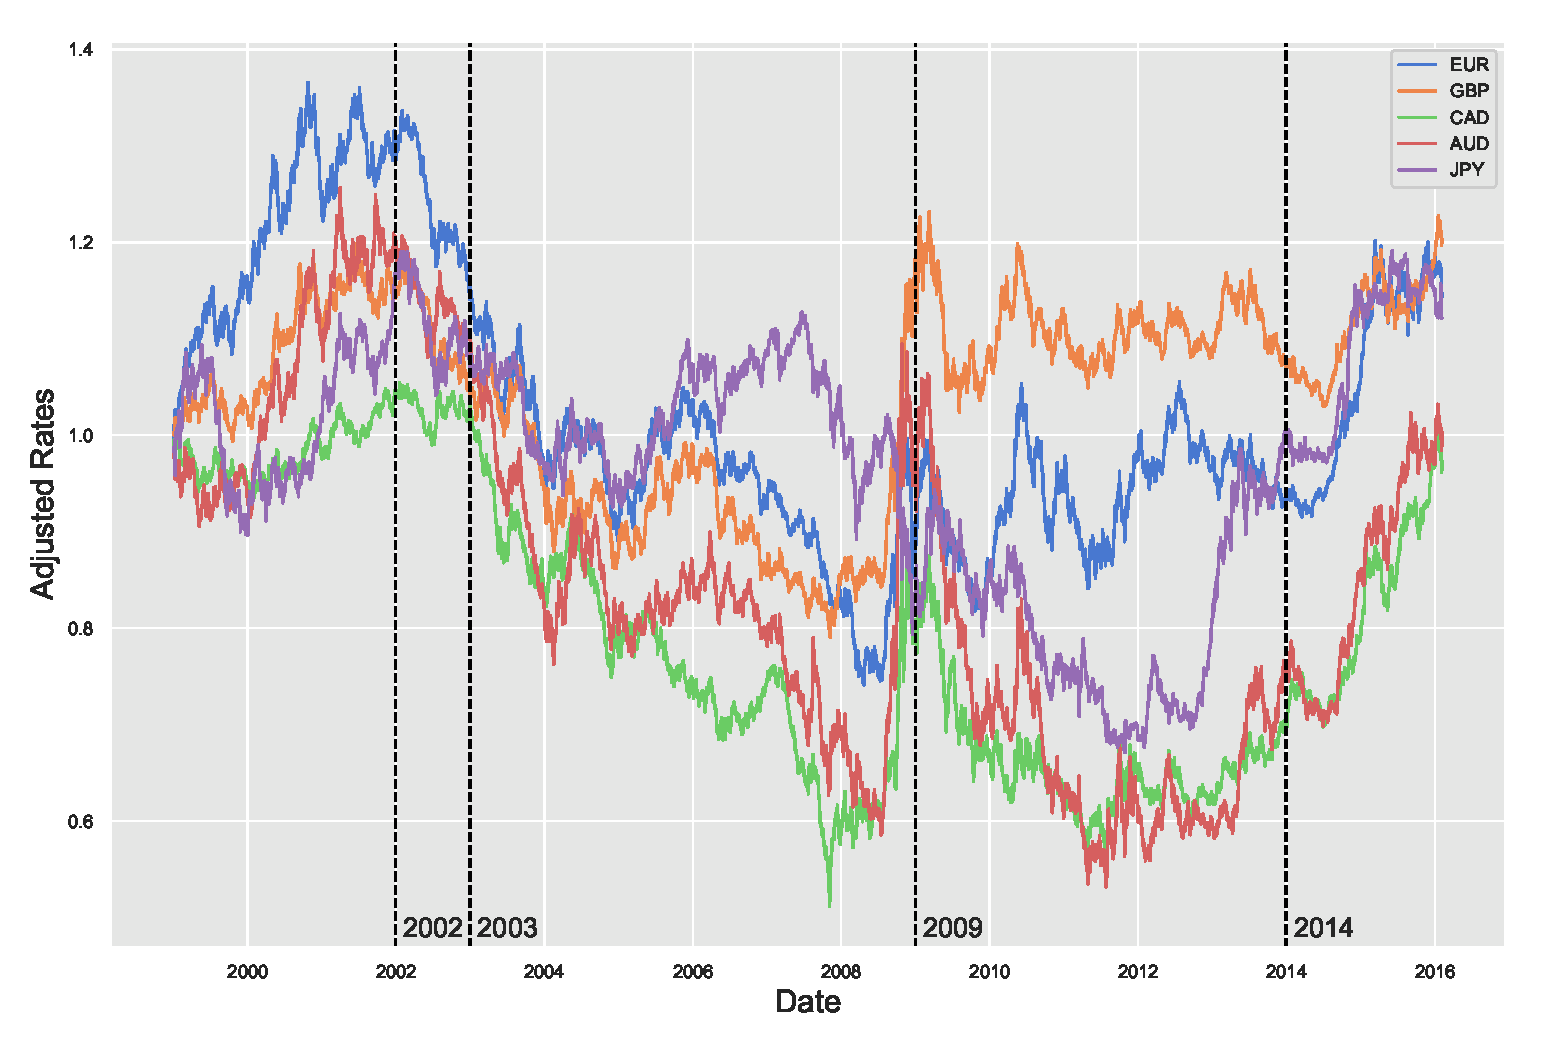
\includegraphics[width=\textwidth]{chapters/chapter_mvts/figures/pexchrate.eps}
	\caption{Plot of Exchange Rates. \label{fig:pexchrate}}
	\end{figure}
	
	\begin{figure}[!ht]
	\centering
	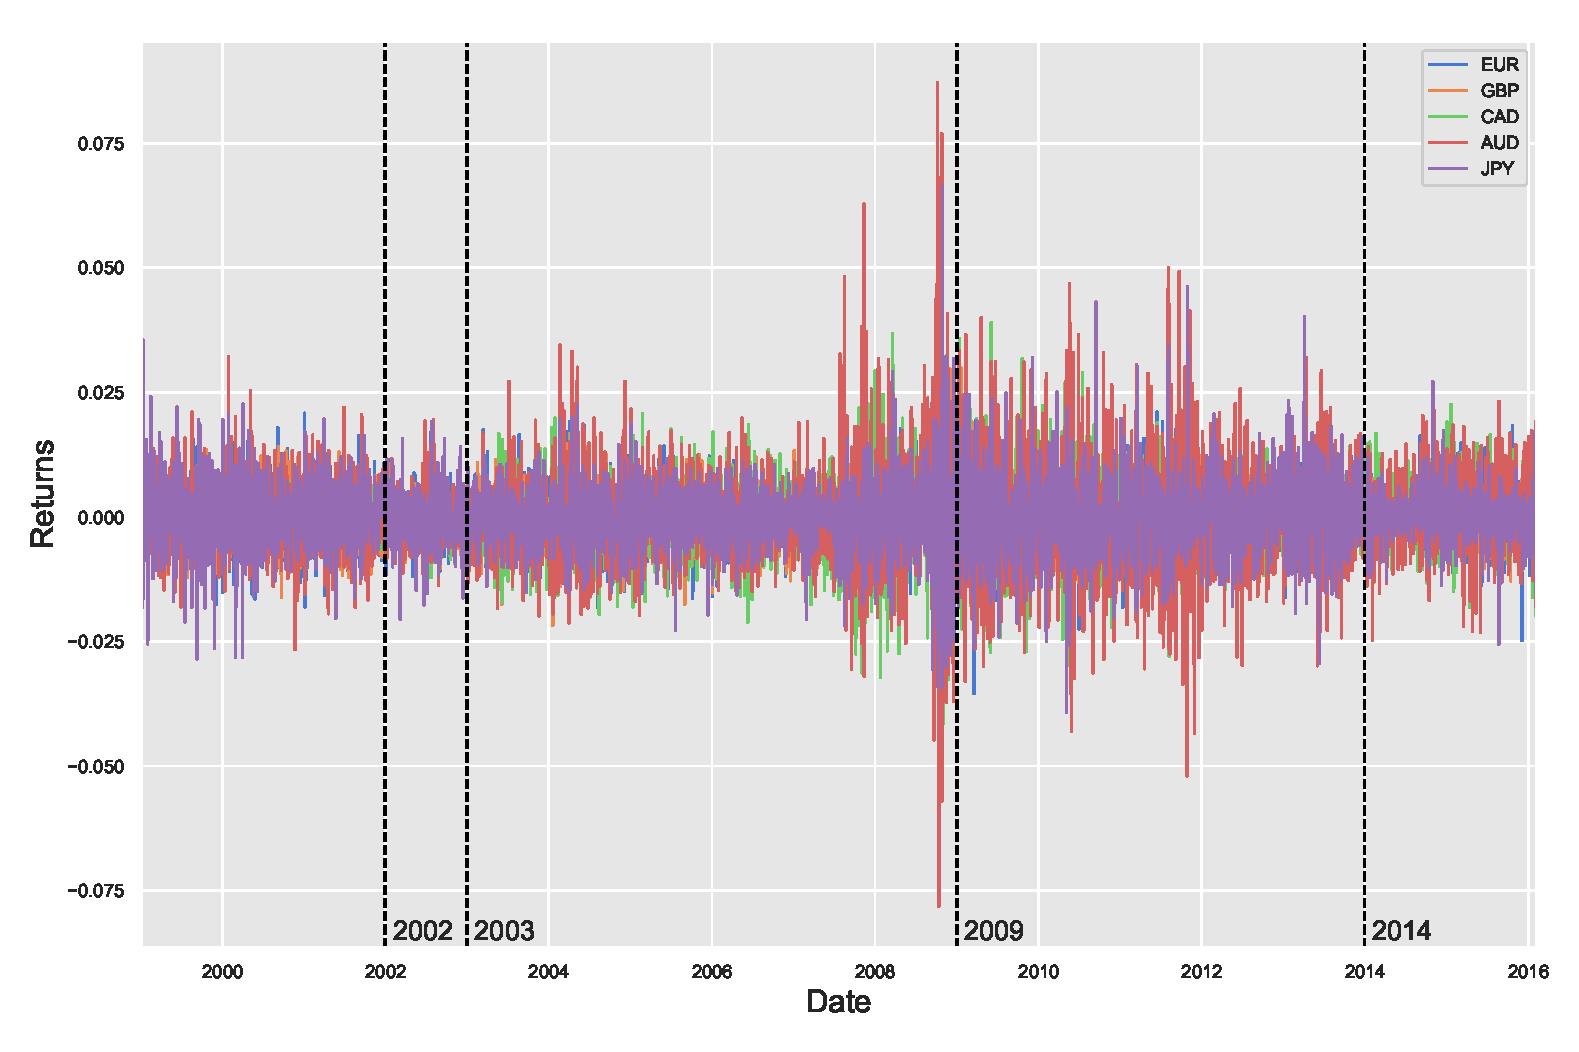
\includegraphics[width=\textwidth]{chapters/chapter_mvts/figures/preturns.eps}
	\caption{Plot of Returns. \label{fig:preturns}}
	\end{figure}
	
	\begin{figure}[!ht]
	\centering
	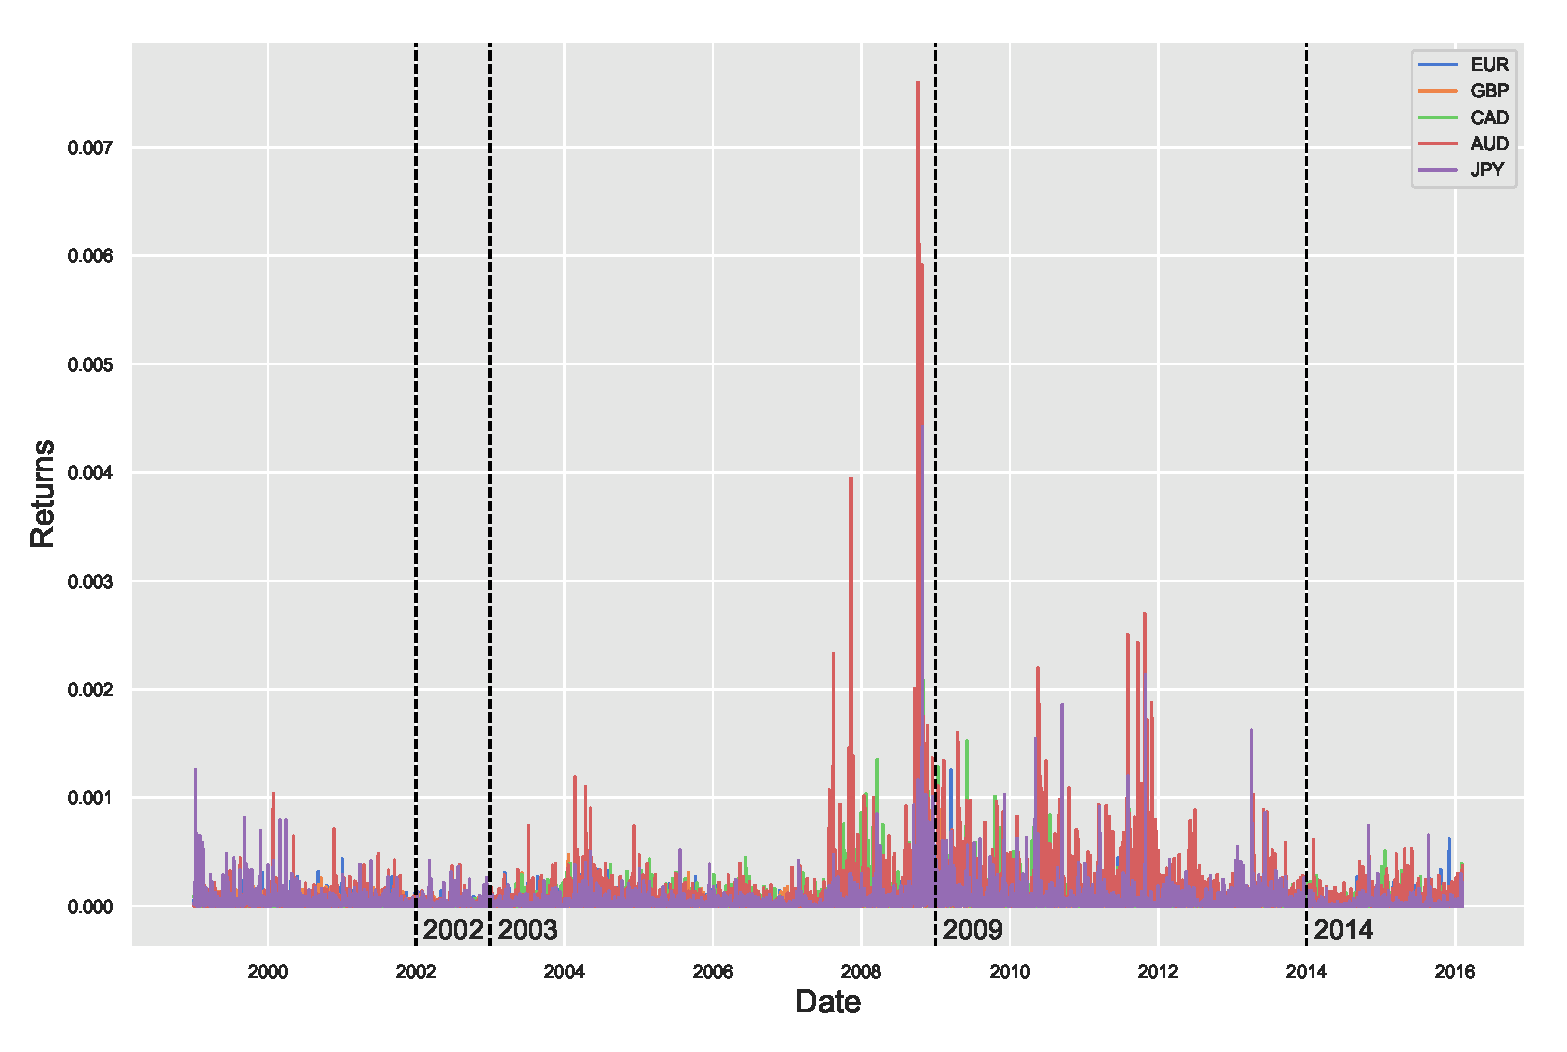
\includegraphics[width=\textwidth]{chapters/chapter_mvts/figures/pvolat.eps}
	\caption{Plot of Volatilities. \label{fig:pvolat}}
	\end{figure}

	\begin{figure}[!ht]
	\centering
	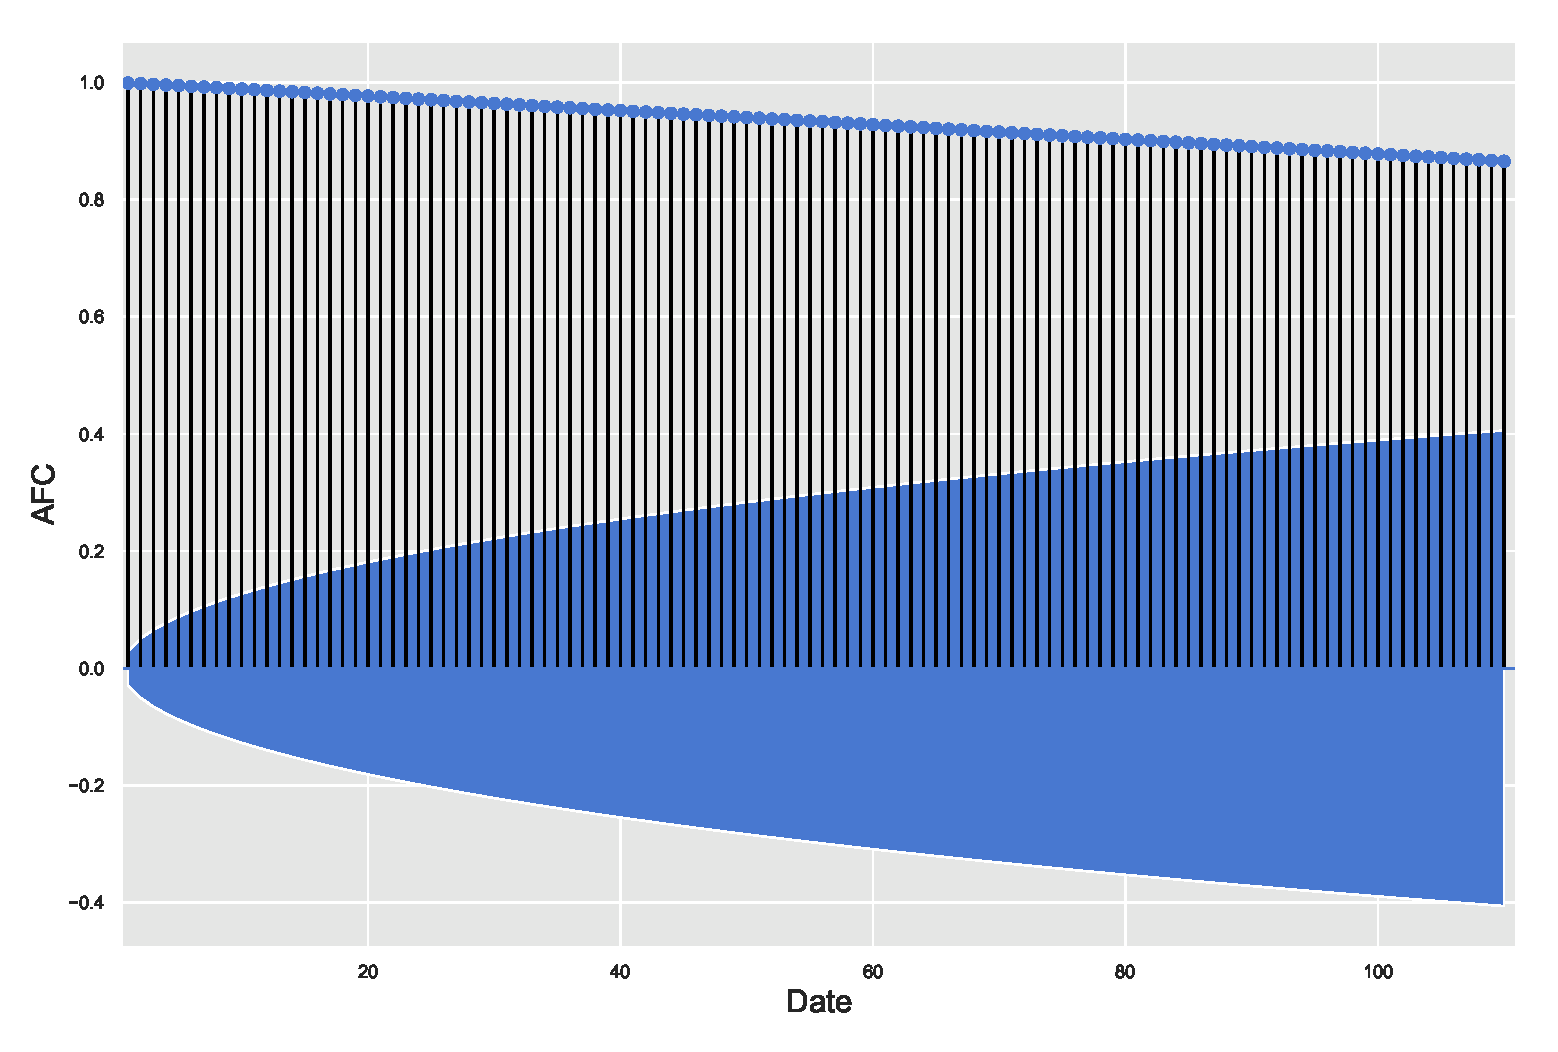
\includegraphics[width=\textwidth]{chapters/chapter_mvts/figures/pautofun.eps}
	\caption{Autocorrelation Function for EUR (with 5\% significance limits for the autocorrelations). \label{fig:pautofun}}
	\end{figure}

	\begin{figure}[!ht]
	\centering
	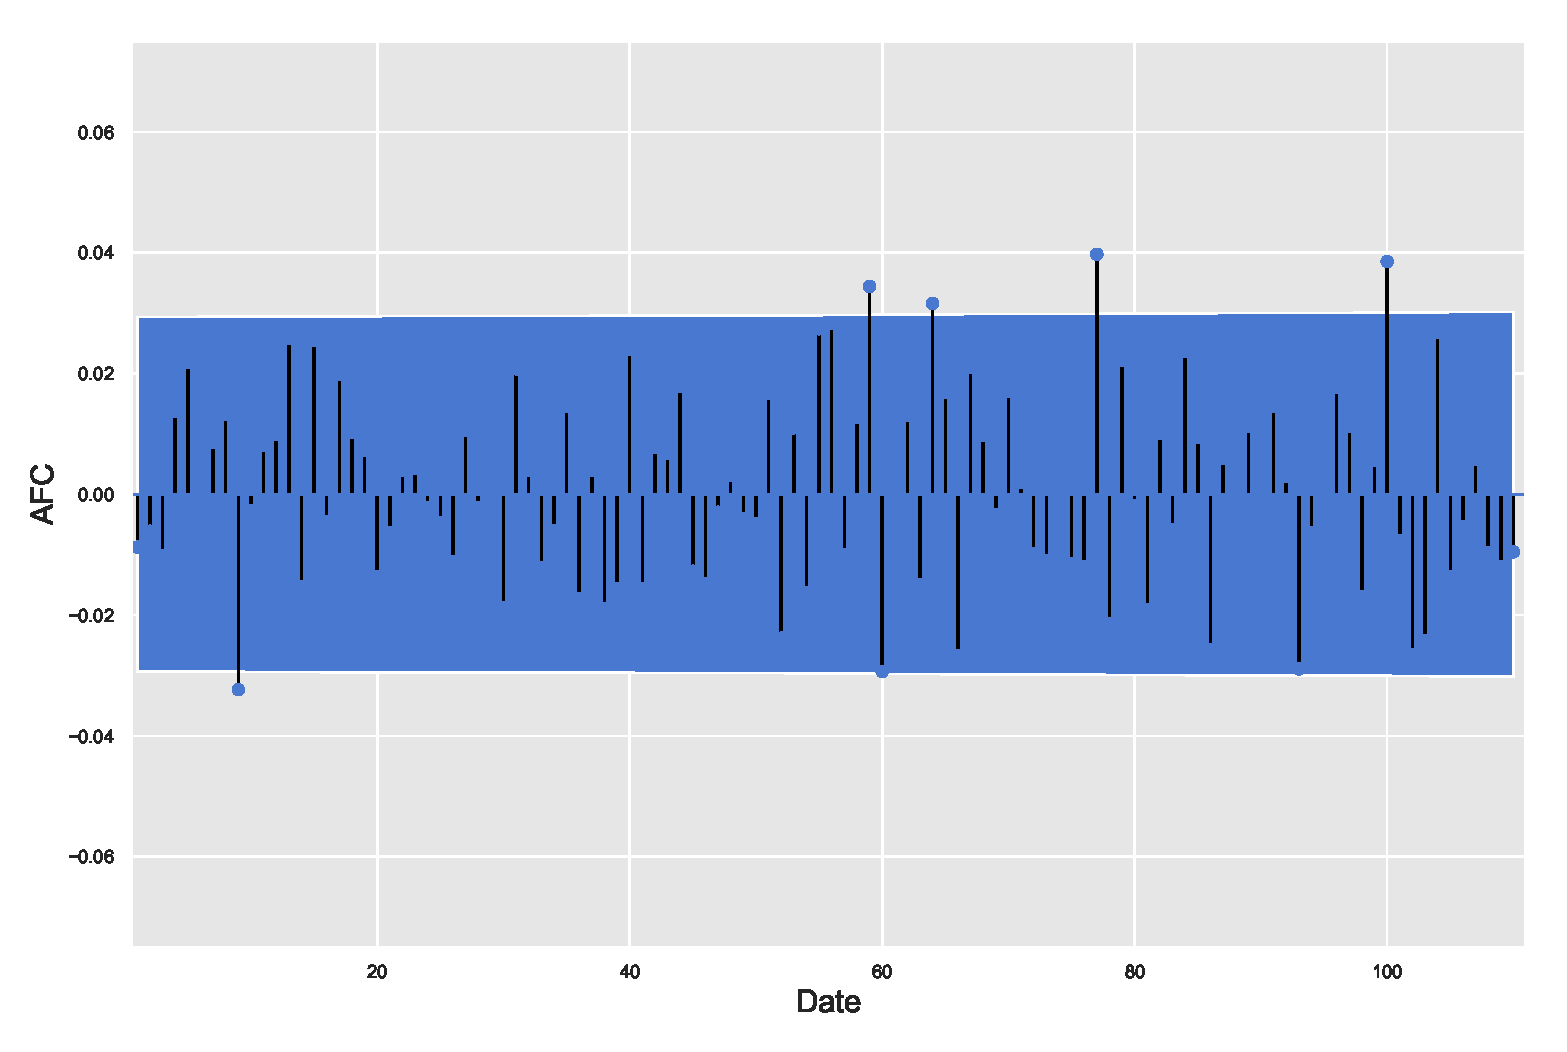
\includegraphics[width=\textwidth]{chapters/chapter_mvts/figures/pautofun2.eps}
	\caption{Autocorrelation Function for EurR (with 5\% significance limits for the autocorrelations). \label{fig:pautofun2}}
	\end{figure}

	\begin{figure}[!ht]
	\centering
	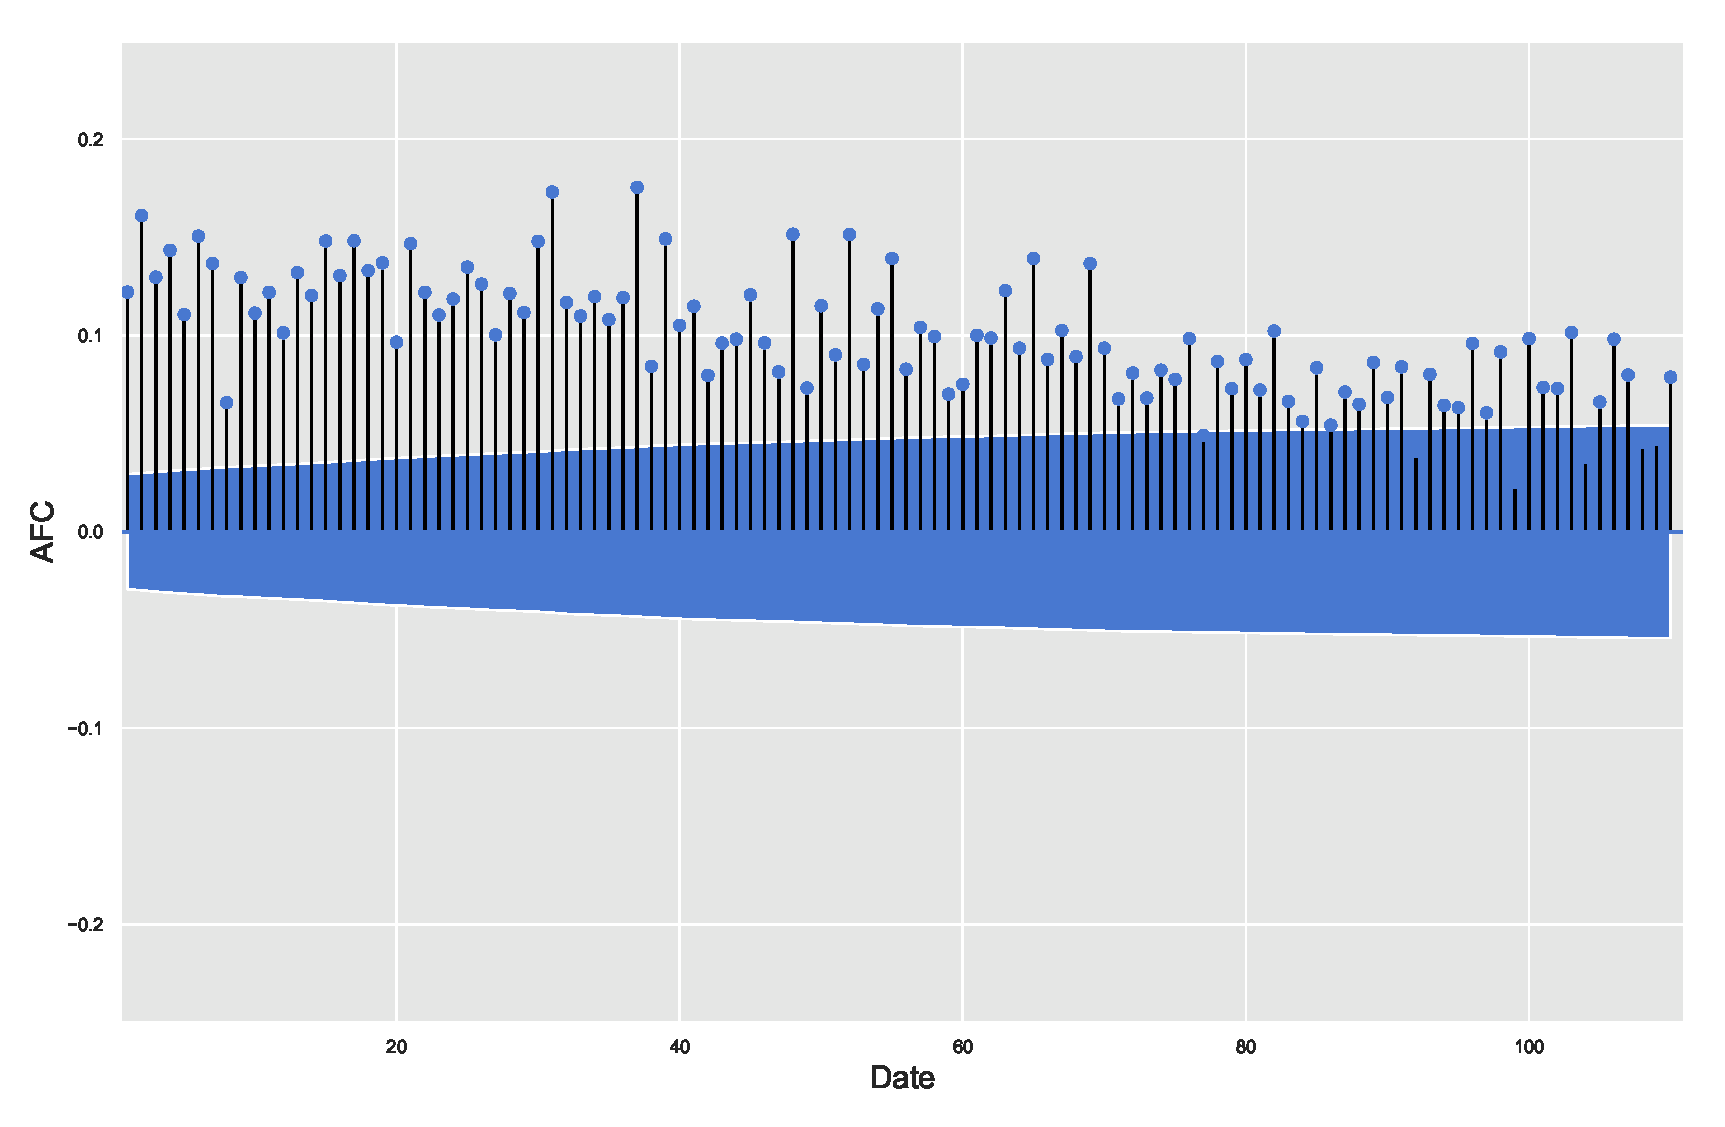
\includegraphics[width=\textwidth]{chapters/chapter_mvts/figures/pautofun3.eps}
	\caption{Autocorrelation Function for EurRSQ (with 5\% significance limits for the autocorrelations). \label{fig:pautofun3}}
	\end{figure}


We want to briefly summarize the main ideas of this chapter. Each component series $y_{it}$ of the vector process $Y_t$ is to be nonstationary with its first difference $(1 - B) y_{it}$ stationary (in which case $y_{it}$ is said to be integrated of order one), but such that certain linear combinations $z_{it} = b_i' Y_t $ of $Y_t$ will be stationary. Then, the process $Y_t$ is said to be \emph{co-integrated} with co-integrating vectors $b_i$ (e.g., Engle and Granger, 1987~\cite{engle1987co}). An elegant interpretation of co-integrated vector series $Y_t$, in Economics, is that the individual components $y_{it}$ share some common nonstationary components or ``common trends'' and, hence, they tend to have certain similar movements in their long-term behavior. A related interpretation is that the component series $y_{it}$, although they may exhibit nonstationary behavior, satisfy (approximately) a long-run equilibrium relation $b_i' Y_t \approx 0$ such that the process $z_{it} = b_i' Y_t$, which represents the deviations from the equilibrium, exhibits stable behavior and so is a stationary process. This is the basis of `pairs trading' discussed in Chapter~\ref{ch:stat_ts}. For a VAR($p$) model, see the discussion in Section~\ref{sec:comts}.


The main steps involved in VAR($p$) modeling are:
	\begin{enumerate}[--]
	\item Identification of the order `$p$' of the process either by examining the significance of the elements of the cross-correlation matrix, $\rho(l)$ for various values of `$l$' or by using one of the criteria, AIC or BIC in \eqref{eqn:2aicbic}.
	\item For the non-stationary VAR, run Dickey--Fuller test \eqref{eqn:hattaunew} to check if individual series are non-stationary. Then build the model in \eqref{eqn:2WtABY}, by first testing the co-integrating rank. 
	\end{enumerate}
[All these calculations can be done by using the `$R$' programs, urca, MTS, fUnitRoots]


The results for the testing co-integration for the full duration and the regime (2008--2009) are presented in Table~\ref{tab:fulldur} and Table~\ref{tab:fulldur2}, respectively. All the other regimes have the same pattern as the full duration and therefore the details are omitted. Except for the regime (2008--2009) we did not find any co-integrating relationships. This probably indicates that the exchange rate series may be moving on their own with no co-dependence. For the regime that is isolated here, the co-integrating relationships are plotted in Figure~\ref{fig:cointser}; there is only \underline{one} stationary transformed series.


	\begin{figure}[!ht]
	\centering
	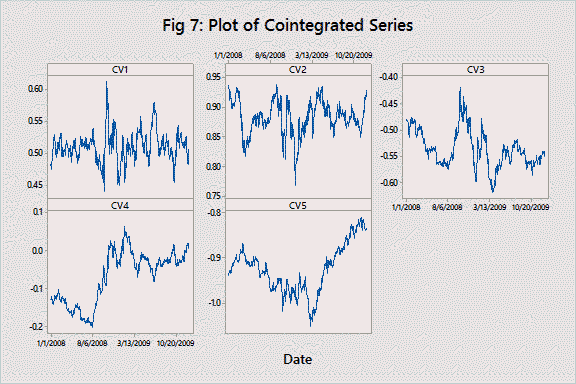
\includegraphics[width=\textwidth]{chapters/chapter_mvts/figures/pcointser.png}
	\caption{Plot of Co-integrated Series. \label{fig:cointser}}
	\end{figure}
	
	\begin{table}[!ht]
	\caption{Full Duration \label{tab:fulldur}}
	\centering
	Eigenvalues ($\lambda$): 0.0054, 0.0030, 0.0018, 0.0008, 0.0003

	Values of test statistic and critical values of test for various ranks: \\[0.1cm]
	
	\begin{tabular}{| l | c | c | c | c |} \hline
	$r$  & test & 10pct & 5pct  & 1pct \\ \hline
	$r \leq 4$ &  1.26 & 6.50 & 8.18 & 11.65 \\ \hline
	$r \leq 3$ &  3.71 & 12.91 & 14.90 & 19.19\\ \hline
	$r \leq 2$ &  7.87 & 18.90 & 21.07 & 25.75\\ \hline
	$r \leq 1$ & 13.47 & 24.78 & 27.14 & 32.14\\ \hline
	$r=0$  & 24.19 & 30.84 & 33.32 & 38.78
	\end{tabular}
	
	Eigenvectors, normalised to first column: (These are the co-integration relations) \\[0.1cm]
	
	\begin{tabular}{| l | c | c | c | c | c |} \hline
	          & EUR &   GBP  &   CAD  &   AUD   &  JPY \\ \hline
	EUR & 1.000 & 1.000 & 1.000 & 1.000 & 1.000 \\ \hline
	GBP & $-0.172$ & $-1.105$ & $-1.721$ &  2.163 & $-0.487$ \\ \hline
	CAD & $-0.890$ &  4.537 & $-0.810$ &  0.707 &  1.666 \\ \hline
	AUD & $-0.343$ & $-3.838$ &  0.829 & $-0.431$ &  0.214 \\ \hline
	JPY &  0.305 & $-0.318$ & $-1.300$ & $-2.242$ & 0.889
	\end{tabular}
	\end{table}
	
	\begin{table}[!ht]
	\caption{Regime 2007--2009 \label{tab:fulldur2}}
	\centering
	Eigenvalues ($\lambda$): 0.0592, 0.0367, 0.0298, 0.0039, 0.0038

	Values of test statistic and critical values of test of co-integrating rank: \\[0.1cm]
	
	\begin{tabular}{| l | c | c | c | c |} \hline
	r               &  test & 10pct & 5pct & 1pct\\ \hline
	r $\leq$ 4 &  1.97  & 6.50 &  8.18 & 11.65\\ \hline
	r $\leq$ 3 &  2.01 & 12.91 & 14.90 & 19.19\\ \hline
	r $\leq$ 2 & 15.77 & 18.90 & 21.07 & 25.75\\ \hline
	r $\leq$ 1 & 19.50 & 24.78 & 27.14 & 32.14\\ \hline
	r = 0  & 31.84 & 30.84 & 33.32 & 38.78
	\end{tabular}

	Eigenvectors, normalised to first column: (These are the co-integration relations) \\[0.1cm]
	
	\begin{tabular}{| l | c | c | c | c | c |} \hline
	         &  EUR  &   GBP  &   CAD   &  AUD  &   JPY \\ \hline
	EUR & 1.000 & 1.000 & 1.000 & 1.000 & 1.000 \\ \hline
	GBP & $-0.628$ & 0.392 & $-0.606$ & 0.379 & $-0.241$ \\ \hline
	CAD & 1.733 & $-0.615$ & $-1.009$ & $-1.189$ & $-0.456$ \\ \hline
	AUD & $-0.919$ & $-0.452$  & 0.519  & 0.103 & $-0.588$ \\ \hline
	JPY & $-0.289$  & 0.522 & $-0.500$ & $-0.567$ & $-0.856$
	\end{tabular}
	\end{table}

	
The co-integration results clearly indicate that the relationships among the exchange rate series could be regime-dependent. This is an important consideration when developing trading strategies. Now we want to examine if there is a linear combination of the returns that exhibit low volatility using the principal volatility component method (PVCM). We compute $r_T=\ln Y_t - \ln Y_{t-1}$ be the five-dimensional returns process. The goal of PVCM, it may be recalled, is to find a matrix, $M$, such that
	\begin{equation} \label{eqn:covmatrixM}
	\cov(Mr_t)= M \Sigma_t M= 
	\begin{bmatrix}
	\Delta_t & c_2 \\
	c_2' & c_1
	\end{bmatrix}
	\end{equation}	
with $\Delta_t$ being time-variant but $c_1$ is time-independent. For a forerunner of this idea in the case of $m= 2$, see Engle and Kozicki (1993)~\cite{engle1993testing} and Engle and Susmel (1993)~\cite{engle1993common}. To find $M$, write the generalized kurtosis matrix \eqref{eqn:cumkurt} as
	\begin{equation} \label{eqn:gammakurt}
	\Gamma_k= \sum_{h=1}^k \sum_{i=1}^m \sum_{j=1}^m \cov^2(r_tr_t', r_{i,t-h} \cdot r_{j \cdot t-h}).
	\end{equation}	


\noindent\underline{Result:} If $r_t$ is a $m$-dimensional stationary series; the ARCH dimension of $r_t$ is $'r'$ if and only if $\rank(\Gamma_\infty)= r$ and the no-ARCH transformation, satisfies, $M \Gamma_\infty= 0$. Essentially, $M$ is the matrix composed of the eigenvectors of $\Gamma_\infty$.


For the five exchange rate series, the computational details are presented in Table~\ref{tab:pvctable}. It can be seen that the last two eigenvalues are fairly small. The linear combinations, $Mr_t$ are plotted in Figure~\ref{fig:transpvc}. The plot of squared values of the two extremes are plotted in Figure~\ref{fig:volextreme}. The autocorrelation functions of the transformed series are plotted in Figure~\ref{fig:autooverall} a \& b; the combination, $0.6835 \text{ EURR} + 0.2054 \text{ GBPR} - 0.3271 \text{ CADR} + 0.1496 \text{ AUDR} + 0.6010 \text{ JPYR}$ exhibits the lowest volatility. It will be interesting to test this out over different regimes.

	\begin{figure}[H]
	\centering
	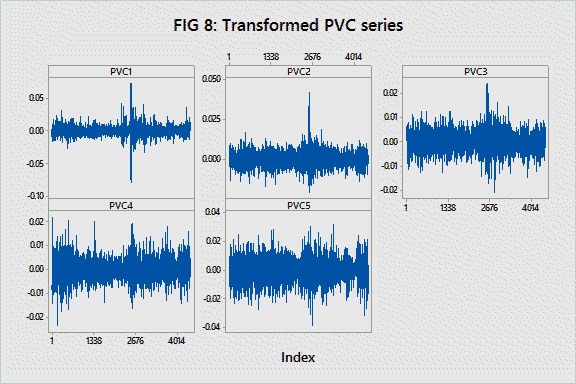
\includegraphics[width=\textwidth]{chapters/chapter_mvts/figures/transpvc.png}
	\caption{Transformed PVC Series. \label{fig:transpvc}}
	\end{figure}


	\begin{figure}[H]
	\centering
	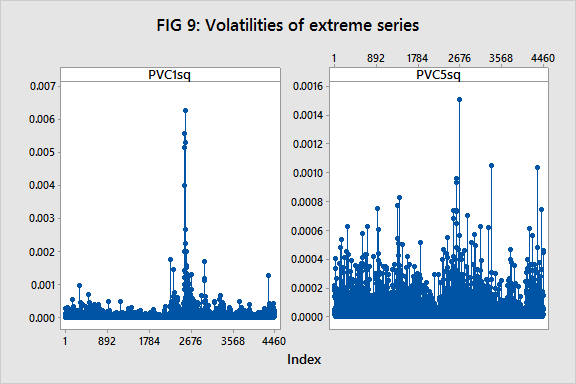
\includegraphics[width=\textwidth]{chapters/chapter_mvts/figures/volextreme.png}
	\caption{Volatilities of extreme series. \label{fig:volextreme}}
	\end{figure}


	\begin{figure}[H]
	\subfloat[Figure 1a]
		[Function for PVC1sq.]
		{
		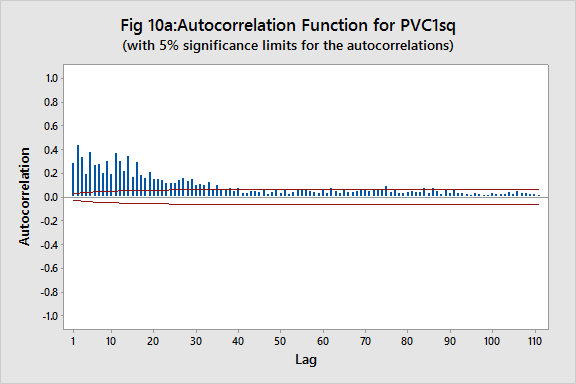
\includegraphics[scale=0.4]{chapters/chapter_mvts/figures/autoa.png}
		}
	\hfill
	\subfloat[Figure 1b]
		[Function for PVC5sq.]
		{
		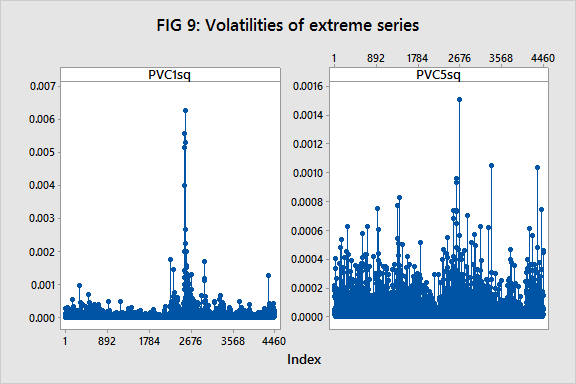
\includegraphics[scale=0.4]{chapters/chapter_mvts/figures/volextreme.png}
		}
	\hfill
	\caption{Autocorrelation Function for PVCs (with 5\% significance limits for the autocorrelations). \label{fig:autooverall}}
            \end{figure}


	\begin{table}[H]
	\centering
	\caption{Principal Volatility Components \label{tab:pvctable}}
	Eigenvalues ($\lambda$): 21.096, 4.453, 1.623, 0.728, 0.435 \\
	
	Eigenvectors
	
	\begin{tabular}{| l | c | c | c | c | c |} \hline
        &    [,1]   &    [,2]    &   [,3]    &   [,4]   &     [,5] \\ \hline
	[1,] & 0.015 & 0.208 & $-0.225$ & $-0.694$ &  0.651 \\ \hline
	[2,] & 0.173 & 0.495 & 0.753 & 0.219 & 0.331 \\ \hline
	[3,] & 0.195 & 0.717 & $-0.577$ & 0.331 & $-0.080$ \\ \hline
	[4,] & 0.859 & $-0.383$ & $-0.114$ & 0.185 & 0.260 \\ \hline
	[5,] & $-0.440$ & $-0.228$ & $-0.191$ & 0.571 & 0.626 \\
	\end{tabular}
	
	$M$--Matrix \\[0.1cm]
	
	\begin{tabular}{| l | c | c | c | c | c |} \hline
	         &   [,1]   &     [,2]    &     [,3]   &    [,4]   &    [,5] \\ \hline
	[1,] & $-0.196$ & 0.077 & $-0.283$ & $-0.755$ & 0.684 \\ \hline
	[2,] & 0.128 & 0.437 & 0.793 d & 0.319 & 0.205 \\ \hline
	[3,]& $-0.070$ & 0.713 & $-0.520$ & 0.321 & $-0.327$ \\ \hline
	[4,] & 0.849 & $-0.512$ & $-0.002$ & 0.129 & 0.150 \\ \hline
	[5,] & $-0.468$ & $-0.180$ & $-0.142$ & 0.455 & 0.601 \\
	\end{tabular}
	\end{table}



% Exercises
\section{Exercises}


% Problem
\prob
\begin{itemize}
\item The file {\tt d\_15stocks.csv} and {\tt m\_15stocks.csv} contain daily and monthly stock returns data for 15 stocks from Jan 11, 2000 to Mar 31, 2013.
\item The file {\tt d\_indexes.csv} and {\tt m\_indexes.csv} contain daily and monthly returns data for the volume-weighted and equal-weighted S\&P500 market indices (VWRETD and EWRETD, respectively) from Jan 11, 2000 to Mar 31, 2013.
\end{itemize}

Using daily and monthly returns data for 15 individual stocks from {\tt d\_15stocks.csv} and {\tt m\_15stocks.csv}, and the equal-weighted and value-weighted CRSP market indexes (EWRETD and VWRETD, respectively) from {\tt d\_indexes.csv} and {\tt m\_indexes.csv}, perform the following statistical analyses using R. For the subsample analyses, split the available observations into equal-sized subsamples.

\begin{enumerate}[(a)]
\item Compute the sample mean $\hat\mu$, standard deviation $\hat{\sigma}$, and first-order autocorrelation coefficient $\hat{\rho}(1)$ for daily simple returns over the entire sample period for the 15 stocks and two indexes. Split the sample into 4 equal subperiods and compute the same statistics in each subperiod---are they stable over time?
\item Plot histograms of daily simple returns for VWRETD and EWRETD over the entire sample period. Plot another histogram of the normal distribution with mean and variance equal to the sample mean and variance of the returns plotted in the first histograms. Do daily simple returns look approximately normal? Which looks closer to normal: VWRETD or EWRETD?
\item Using daily simple returns for the sample period, construct 99\% confidence intervals for $\hat{\mu}$ for VWRETD and EWRETD, and the 15 individual stock return series. Divide the sample into 4 equal subperiods and construct 99\% confidence intervals in each of the four subperiods for the 17 series---do they shift a great deal?
\item Compute the skewness, kurtosis, and studentized range of daily simple returns of VWRETD, EWRETD, and the 15 individual stocks over the entire sample period, and in each of the 4 equal subperiods. Which of the skewness, kurtosis, and studentized range estimates are statistically different from the skewness, kurtosis, and studentized range of a normal random variable at the 5\% level? For these 17 series, perform the same calculations using monthly data. What do you conclude about the normality of these return series, and why? \twomedskip
\end{enumerate}


% Problem
\prob For the data in Exercise~1, carry out the following:

\begin{enumerate}[(a)]
\item Perform a PCA on the 15-stock returns. Using the eigenvalues of the $\hat{\Sigma}$ matrix, identify the number of factors.
\item Compute the covariance between the returns and the factors and comment. \twomedskip
\end{enumerate}


% Problem
\prob Consider the weekly exchange rate data used in Hu and Tsay (2014)~\cite{hutsay14}: British Pound ($y_{1t}$), Norwegian Kroner ($y_{2t}$), Swedish Kroner ($y_{3t}$), Swiss Franc ($y_{4t}$), Canadian Dollar ($y_{5t}$), Singapore Dollar ($y_{6t}$) and Australian Dollar ($y_{7t}$) against US Dollar from March 22, 2000 to October 26, 2011.

\begin{enumerate}[(a)]
\item Test if the exchange rates are stationary individually via Dickey-Fuller test.
\item Test for co-integration using the likelihood-ratio test given in \eqref{eqn:2negT}. Assume that the order of the VAR model as, $p= 2$.
\item Compute the log returns: $r_t= \ln(Y_t) - \ln(Y_{t-1})$; Fit VAR(5) model for the returns and extract the residuals. 
\item Using the residuals from (c), compute the $\Gamma_k$ matrix in \eqref{eqn:cumkurt} for $k= 5, 10, 20$ and obtain the $M$-matrix in \eqref{eqn:obtainM}.
\item Plot $MY_t$ and comment on the linear combination that has low volatility. 
\item Check (a)--(e) for various regimes; note 2008--2009 is noted for its volatility. 
\end{enumerate}